\chapter{Dynamic Map Design and Development}
\label{chap:softdev}

\chapterquote{It should be trivial.}
{Dr. Robert S Laramee, 2016}

\newpage
{\footnotesize \hypersetup{linkcolor=black}
\minitoc} \newpage

\section{Introduction and Motivation}
Throughout the course of this thesis, we implemented two software-driven chapters as well as a user-study developed using custom software. There are many design challenges and obstacles that ocurred throughout the development of software components and this chapter highlights some of the major themes. We focus on three specific topics for this chapter: debug visualization, geometric primitive testing, and the complexities of boundary identification.
When creating complex algorithms for diverse data sets, there are many opportunities for errors or oversights to present themselves. Even when we discover them, it can be difficult to determine the cause without efficient debugging strategies. This concept is important when working with geospatial data.
We present some debug visualization techniques that are used to process the representation of geospatial data for the dynamic choropleth map algorithm (Chapters \ref{chap:dcm}, \ref{chap:userStudy}, and \ref{chap:MultivariateMaps}).



\section{Background}
In 1981, Baecker presented the `Sorting Out Sorting' case study, a visual comparion of many sorting algorithms for different test cases.The paper was aimed at teaching user when to use which sorting algorithms with the help of animation. \cite{baecker1981sorting, baecker1998sorting}. This concept was extended upon by Brown and Sedgewick who present BALSA (Brown ALgorithm Simulator and Animator) \cite{brown1984system}.
Eisenstadt and Brayshaw design the transparent prolog machine (TPM), a visual debugger for logic programming. The software include a viewport control panel, allowing the user to step through the logic at intervals, reset the logic, or play the as an animation. TPM also allowed the user to interact with the visualization such as highlighting nodes \cite{eisenstadt1988transparent}. 
Lehr et al.\ review visual performance debugging in the form of PIE (Parallel Programming and Instrumentation Environment). The software provides visualization to sense how parallel execution. A comparison of three different Kernals are compared to understand how the execution differs \cite{lehr1989visualizing}.
Price et al.\ present a taxonomy looking at tweleve types of software visualization including both algorithm visualization and program visualization \cite{price1993principled}.
Tal and Dobkin present a visual debugging framework named GASP (Geometric Animation System, Princeton). GASP aims to present a fast reactive system that allows the user to depict and modify geometric shapes with an effective turnaround \cite{tal1995visualization}.
Crossno and Angel present a case study of visual debugging developed for studying particle systems including particle placement and size, neighbour linkage, and triangle generation \cite{crossno1999visual}.
Crossno and Rogers discuss how visual debugging can provide insights that ordinary debugging conventions would not, focusing on scientific visualization \cite{crossno2002visual}.
Ericson provide a useful guide for real-time collision detection with a focus on programming examples and cases \cite{ericson2004real}.
Laramee presents a paper discussing how to use visualization to debug software. We use this as a baseline for our guide, but extend upon this with new concepts with an emphasis on geospatial visualization \cite{laramee2009using}.
Gribble et al.\ present the Ray-tracing Visualization Toolkit (rtVTK) which allows the user to quickly interpret more complex ray-tracing techniques such as recursive properties and path-tracing. This acts as a plugin for the already existing VTK \cite{gribble2012ray}.
Gouveia et al.\ review the use of visualization to detect the location of software faults using GZoltar \cite{campos2012gzoltar}. They find that including one of their three visualizations (sunburst, vertical partition, bubble hierarchy) greatly increases the time to trace the fault in the code base \cite{gouveia2013using}.
Beck et al.\ produce a visual debugging tool for regular expressions. The interface is split into a legend panel, a regular expression implementer in the form of a visually-enhanced text input form, and a second text box to input test cases. The test cases will highlight whether the test is passed or failed with instant attempt-to-response time \cite{beck2014regviz}.
Spencer et al.\ present a tool for the visualization of photon data, used to minimize the amount of error presented by photon mapping. This tool is used to rapidly attempt trials with a quick visual response, differing from our concepts which aid the user in pre-processing steps of geometry manipulation \cite{spencer2015visualization}. 

%Although Laramee has already presented some work on this topic \cite{laramee2009using}, we extend this with concepts specific to geospatial visualization, and our specific experience.

\section{Debug Geospatial Visualization Concepts}
In this section, we will discuss some concepts which are incremental but still important to efficient debug visualization.
\\ \textbf{Step Function: }One of the most important tools when using debug visualization is the proper use of a step function. A step function is used to stop-and-go through different stages of a visualization process incrementally. In our project, a step function can be toggled on and off using a checkbox. This enables us to check whether the intermediate results are as intended for each section of the algorithm (discussed in the proceeding sub-sections), at each interval (intervals discussed in detail below). 
\\ \textbf{Color Mapping: }It is important to distribute roles clearly using color. Color is an essential tool in any visualization and debugging is no exception. For our algorithm, we used grey to signify context and blue to signify the focus of the current processing step. If there is no obvious way of determining the number of colors needed, the use of seeded colors can be useful. This is shown in Section \ref{sec:contigVis}.
\\ \textbf{Test Data sets: }Testing an algorithm on multiple data sets is a key aspect of debugging your software and is a concept not exclusive to the visualization process of debugging. We worked with over ten test example data sets. These datasets are split into smaller, more manageable sub-sets. The data sets ranged from 20 polygons up to over 30,000 polygons. If an error occurred during the algorithm run, the area in which the error occurred was identified, investigated and split into a smaller data set to add to our test runs.
\\ \textbf{Comparative Software: }Software that handles similar data can be an essential tool in interpreting errors. We thank QGIS \cite{qgis2015qgis} for helping us understand why errors may occur, and what should be expected from the test data sets.
\\ \textbf{Multiple Views: }In order to gain the most out of our debug visualization, we enable two different viewpoints to be toggled. The first viewpoint we used is an overview which presents the map in full. This allows the user to understand how far the algorithm has progressed accurately. We also allow the user to move the extents to follow the current processing step's result, which we identify as a focus processing step. This allows for a clearer representation of the current processing step, letting us observe errors quickly. Using both of these views are  essential in the progression of the algorithm. Figures \ref{fig:hierarchyOverall} and \ref{fig:hierarchyFocus} are examples of how the views can differ during the debug process.

\section{Overview}
Since our debug visualization is communicated in our pre-processing steps. We will present  our overview in a similar fashion to Chapter \ref{chap:dcm}. To reiterate the procedure. Our first step is to load and normalize the data. We ran into a few errors here, which were adjusted using debug visualization. Identify contiguous regions is the next step of our procedure, splitting contiguous regions into seperated lists. After sorting the areas to improve performance, we begin the hierarchical agglomerative clustering steps which is where the bulk of our problems were found. You can review this procedure in Figure \ref{fig:procedure6}.\\
\begin{figure*}[t] 
\centering
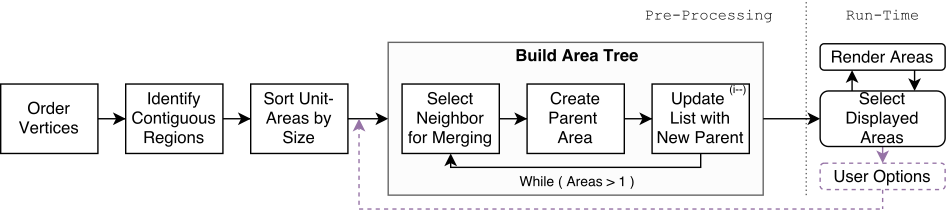
\includegraphics[width=1\textwidth]{images/HorizontalFlow2}
\caption{ The pipeline for the area amalgamation algorithm. After loading the shapefile, polygons are partitioned based on area contiguity, and sorted within islands (or land masses) based on their size. A recursive function is then used to identify new parent areas and their boundaries until their are no remaining neighbors to merge. } \label{fig:procedure6} \vspace{-0.2cm}
\end{figure*}
\textbf{Data Loading Verification: }Debug verification of polygon loading is a simple concept. Each step presented the last loaded polygon mapped to the color blue, while previously loaded areas are rendered as grey context this allows us to see in what order polygons are loaded, which helped us depicts missing polygons. See Figure \ref{fig:loadingMatrix} for a visual representation.\\
\textbf{Contiguity Verification: } We reduce the complexity of hierarchy building by introducing a constraint that all hierarchies are complete when exactly one area remains in our merge candidate list. See Chapter \ref{chap:dcm}. This is done after the areas are loaded. In order to do this, we need to make sure that every instance of the hierarchy is formed as one contiguous region. We debug this aspect by mapping a random color to each list of polygons (representing a contiguous region) at each intermediate step, where a step is presented when each polygon has its contiguity tested. As there may be an arbitrary number of contiguous regions, pre-designating identifiable colors may be difficult. Therefore, in order to address this challenge, we altered the program slightly. When a polygon is assigned to a contiguous region, a new color is assigned to the region, This allows for a visible understanding of the change without the need for the step function. We present a matrix of images showing a concise contiguity visualization in Figure \ref{fig:contigMatrix}. The file represents a test data set taken from the LSOA's of Wales, specifically the contiguous mainland of Anglesy \cite{wales}.\\
\textbf{Area Merge Verification: } In Chapter \ref{chap:dcm}, we state that over 50\% of merges have at least one error case, which is why this section is so important. Our hierarchy building visualization is used to support the identification of a shared boundary between two areas. For each step, we present the newly unified area in blue and every other area that is considered a merge candidate as grey context. This enables us to observe the hierarchy at run time, as well as how it is built. This visualization type enables the user to perceive the majority of errors found during the creation of our algorithm.\\
\textbf{Neighbour Testing Verification: } The final visualization was created as a reaction to some of the errors presented in the area merge verification. In order to clearly identify a selected neighbour, we would highlight the selected merge candidate before the merge was declared. This helped verify that the errors were occuring during the unification of our areas and not the selection process.

\begin{figure}
\begin{tabularx}{1\textwidth}{XXXX}
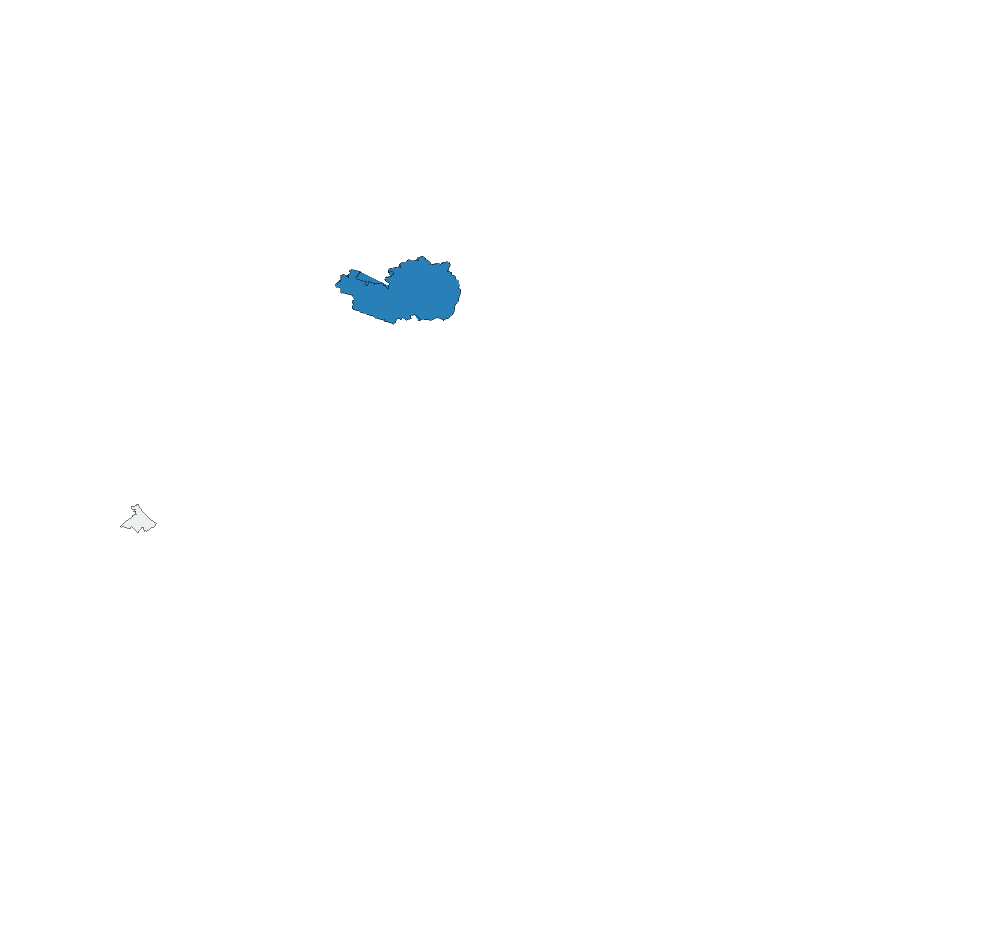
\includegraphics[width=1\linewidth]{images/ch6/loading/01}&
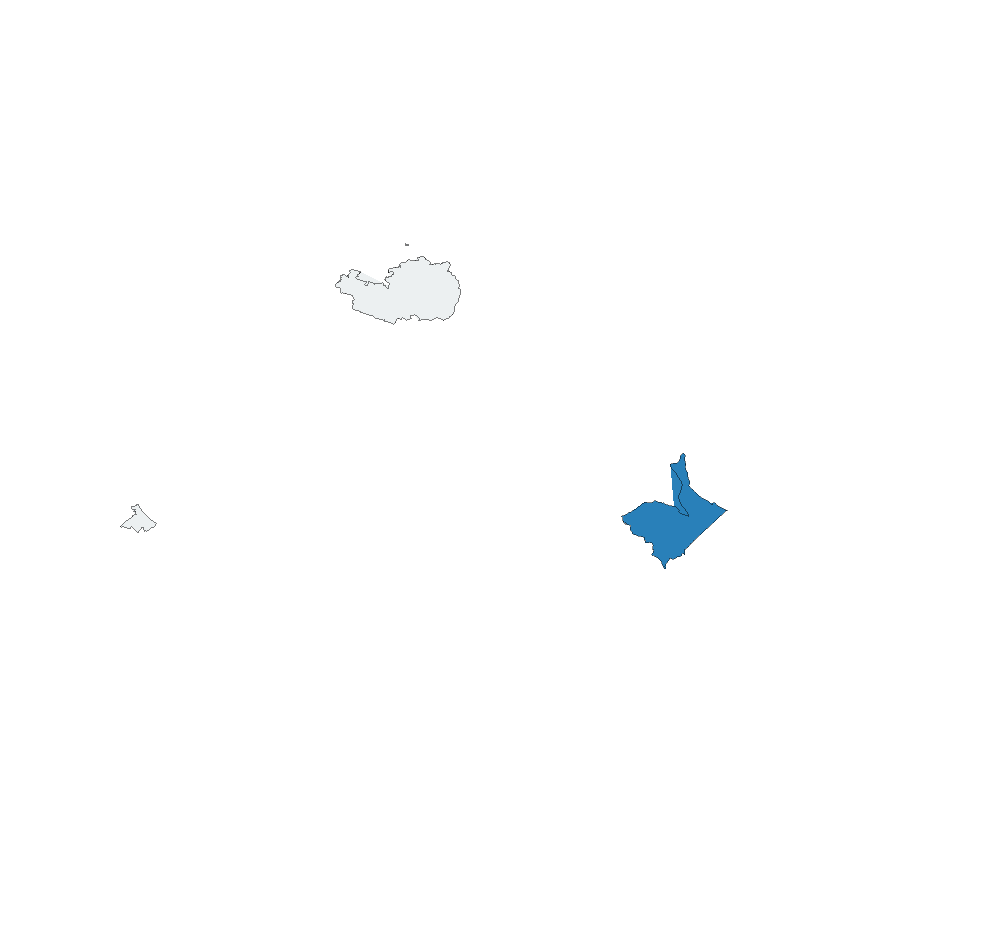
\includegraphics[width=1\linewidth]{images/ch6/loading/02}&
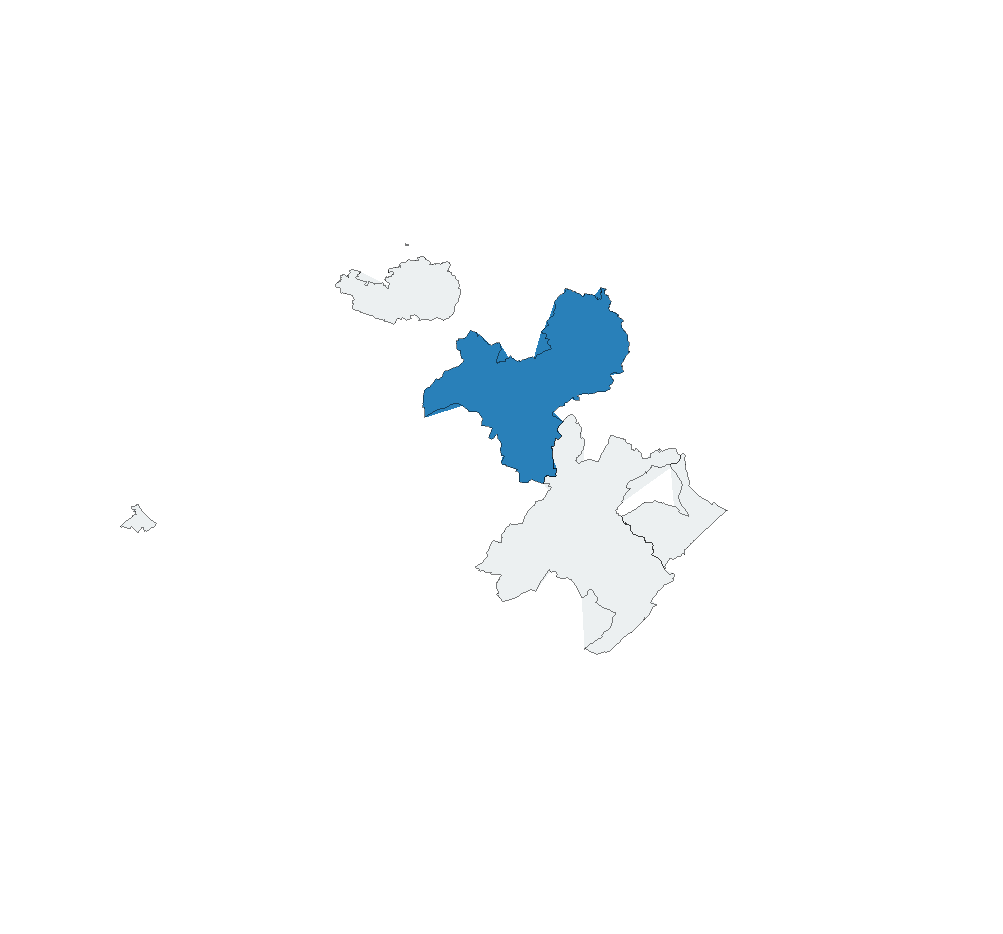
\includegraphics[width=1\linewidth]{images/ch6/loading/03}&
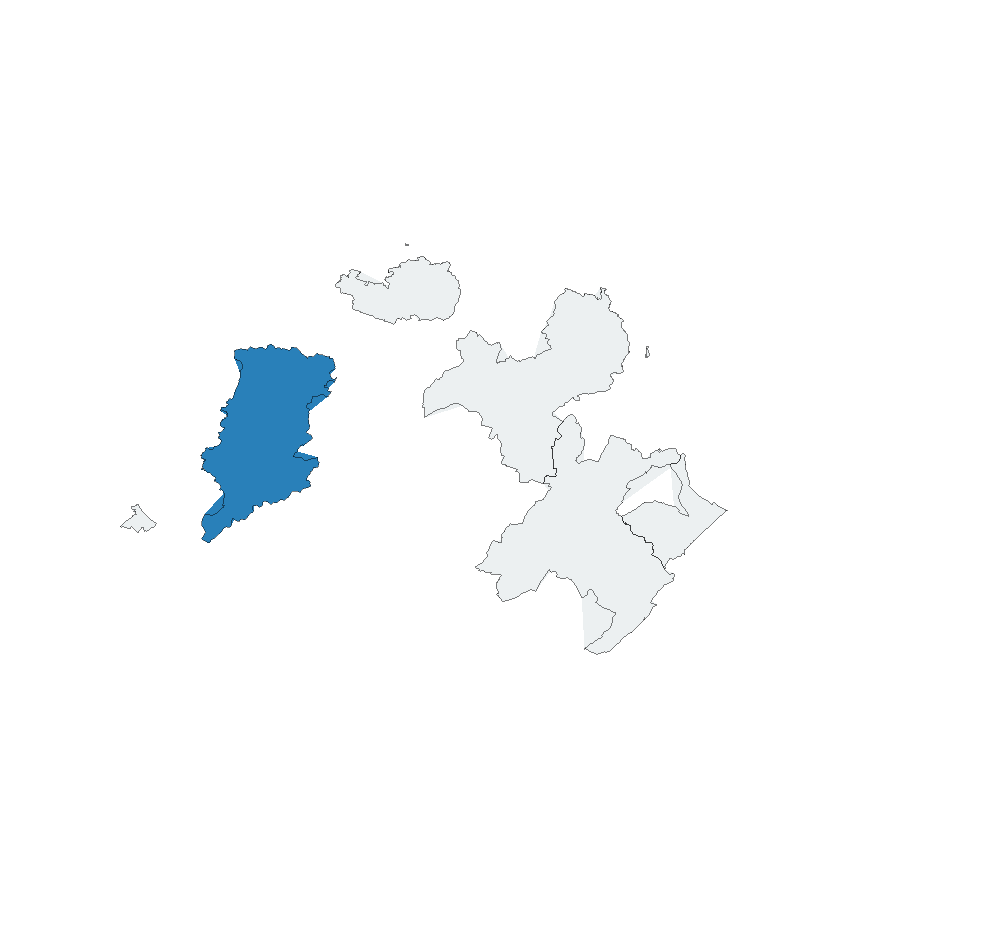
\includegraphics[width=1\linewidth]{images/ch6/loading/04} \\
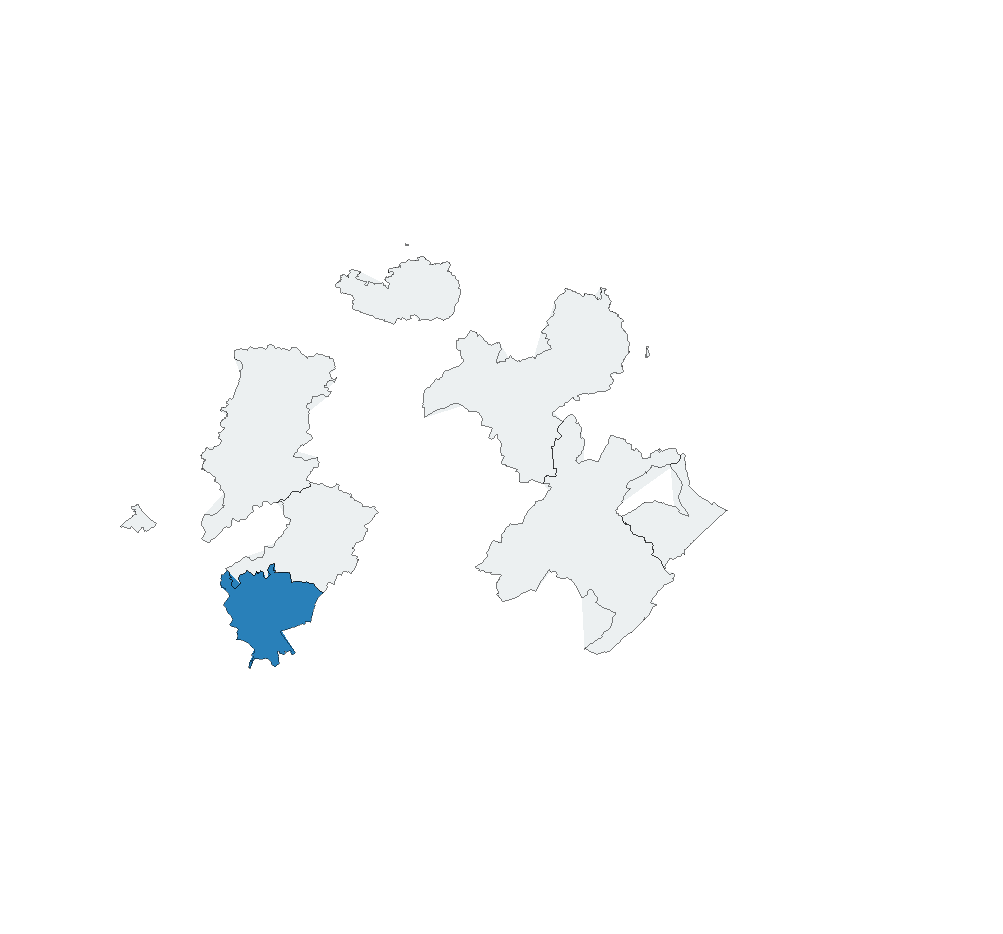
\includegraphics[width=1\linewidth]{images/ch6/loading/05}&
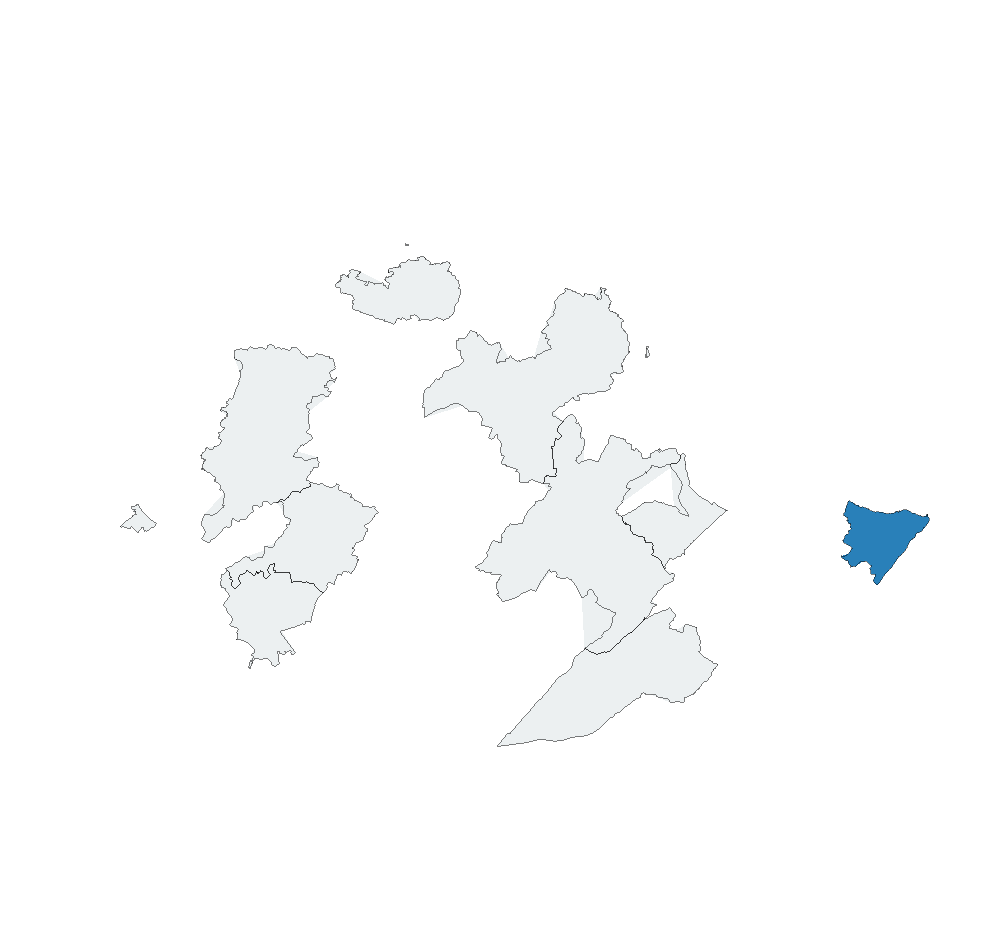
\includegraphics[width=1\linewidth]{images/ch6/loading/06}&
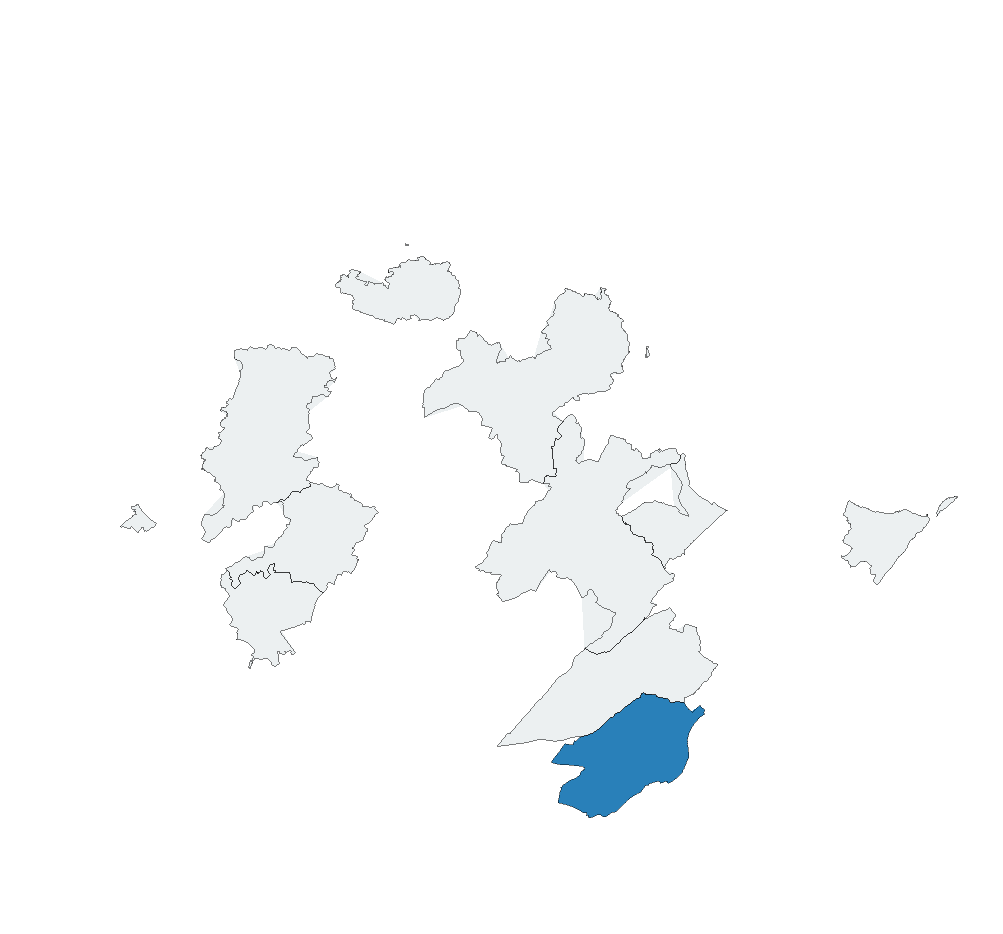
\includegraphics[width=1\linewidth]{images/ch6/loading/07}&
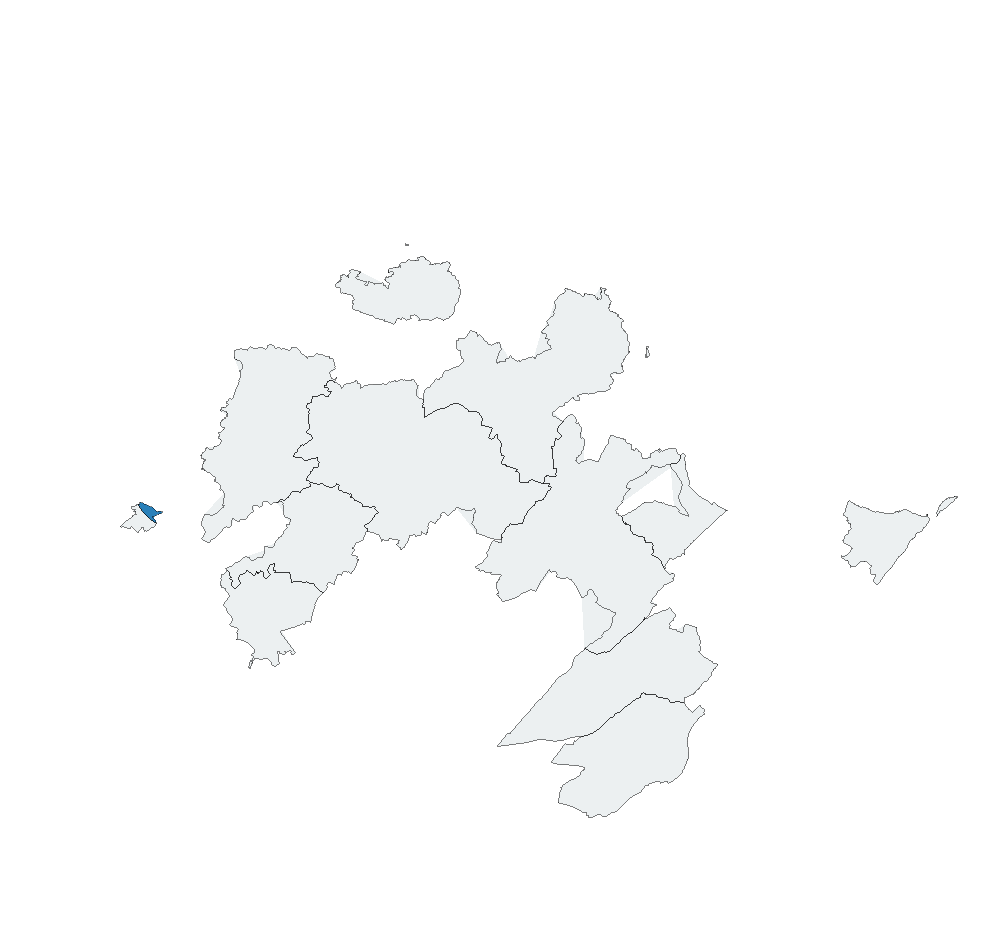
\includegraphics[width=1\linewidth]{images/ch6/loading/08} \\
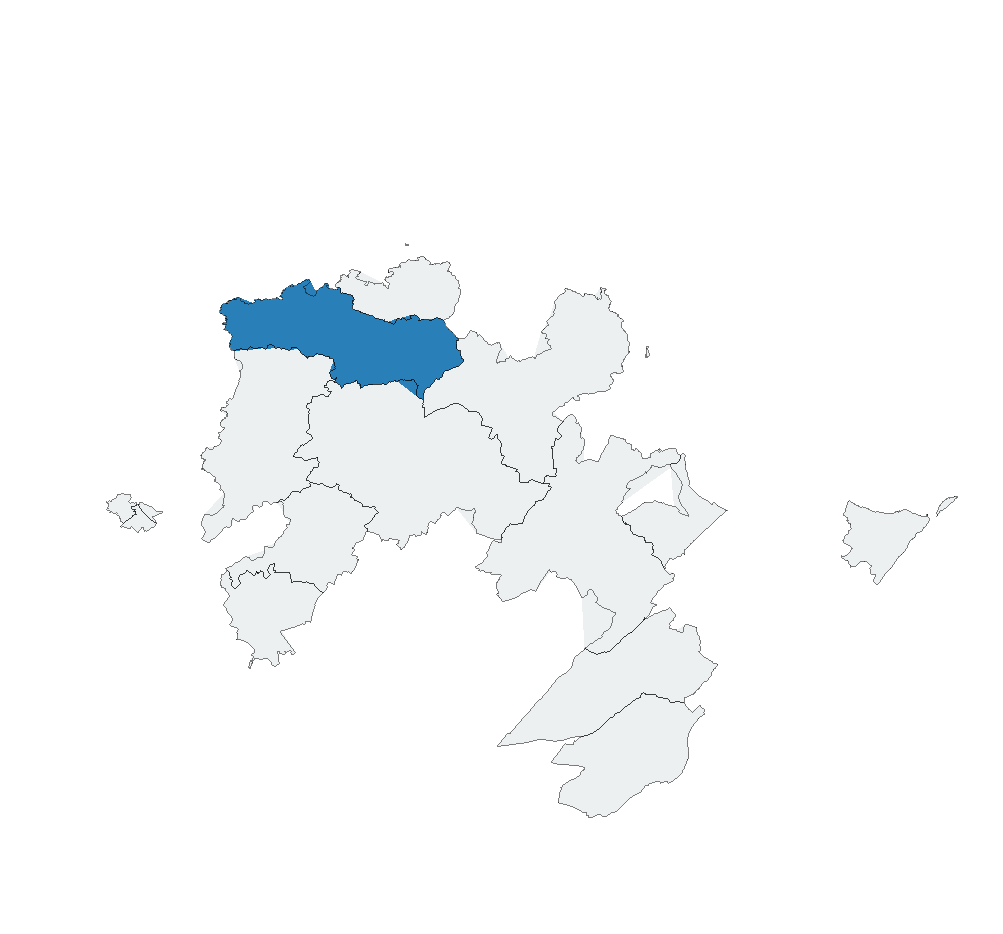
\includegraphics[width=1\linewidth]{images/ch6/loading/09}&
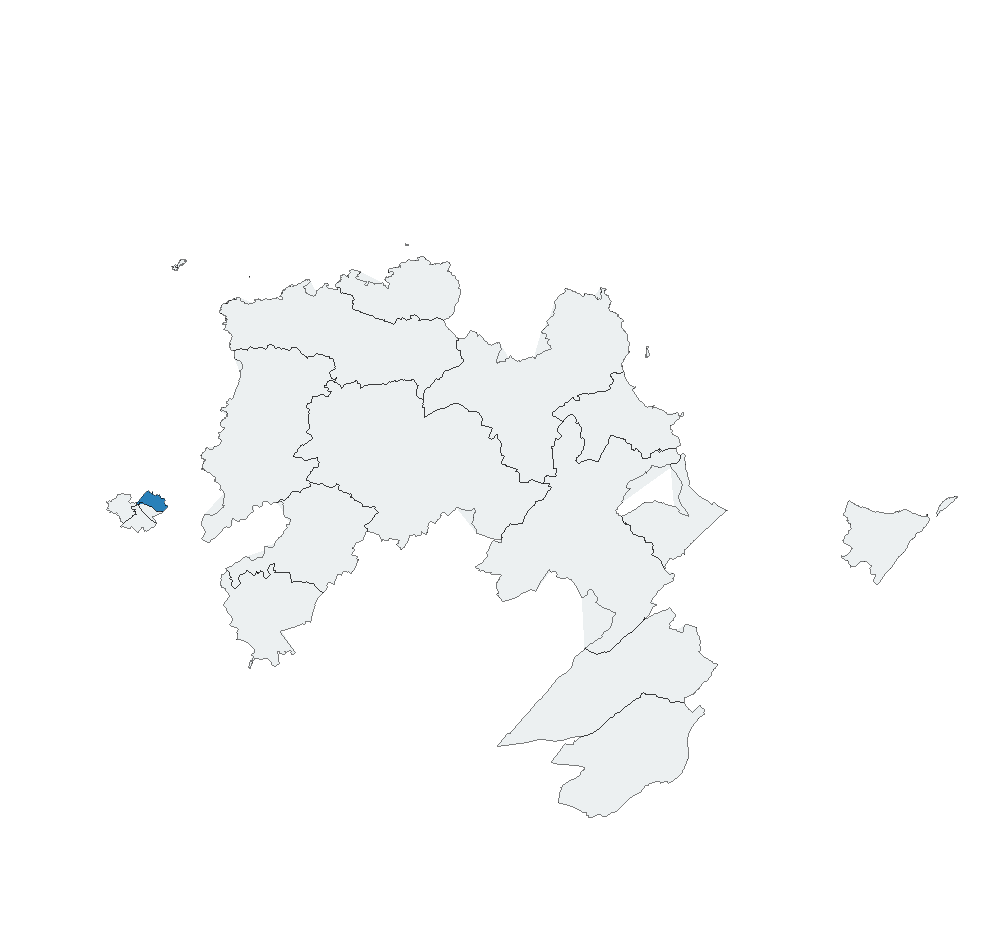
\includegraphics[width=1\linewidth]{images/ch6/loading/10}&
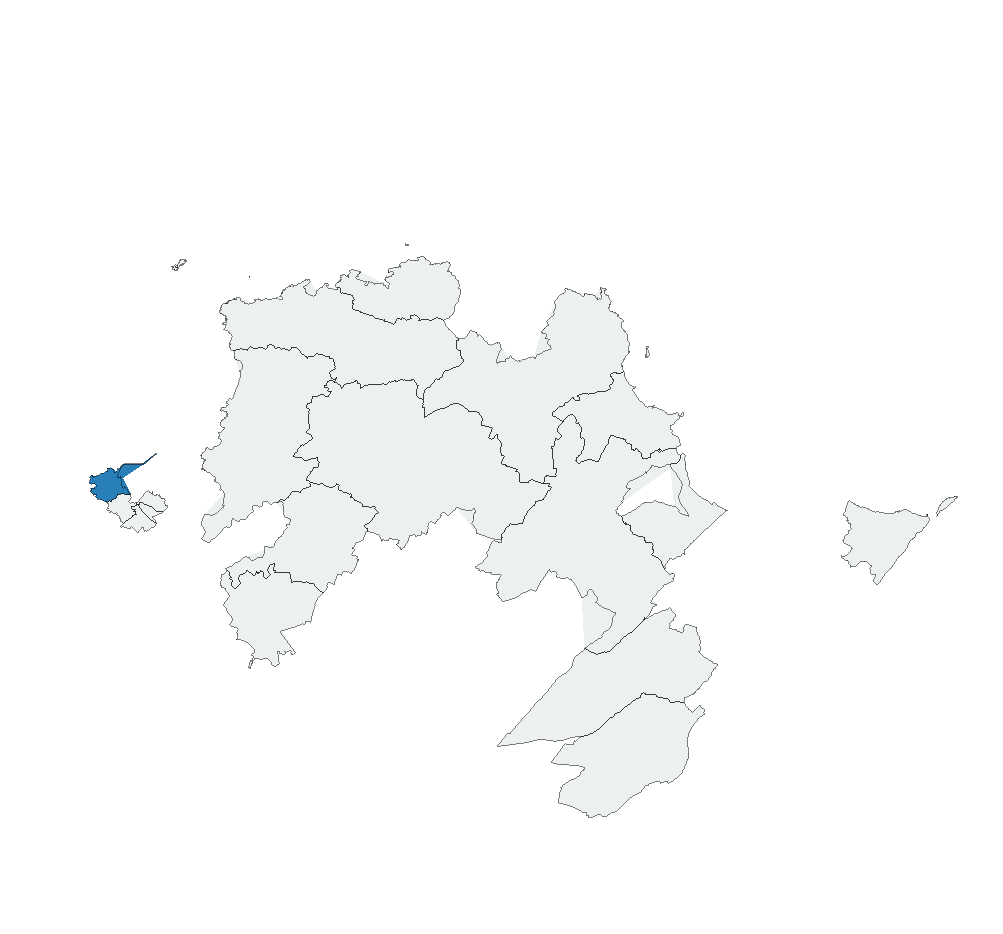
\includegraphics[width=1\linewidth]{images/ch6/loading/11}&
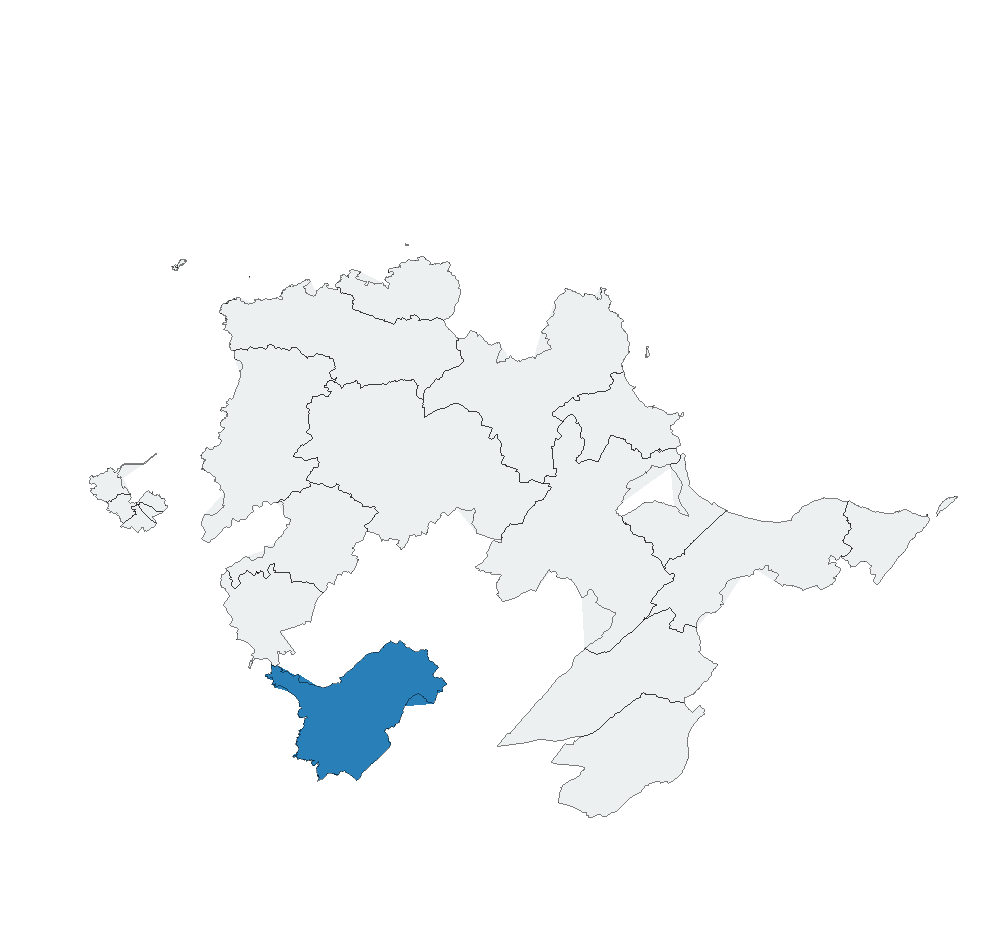
\includegraphics[width=1\linewidth]{images/ch6/loading/12} \\
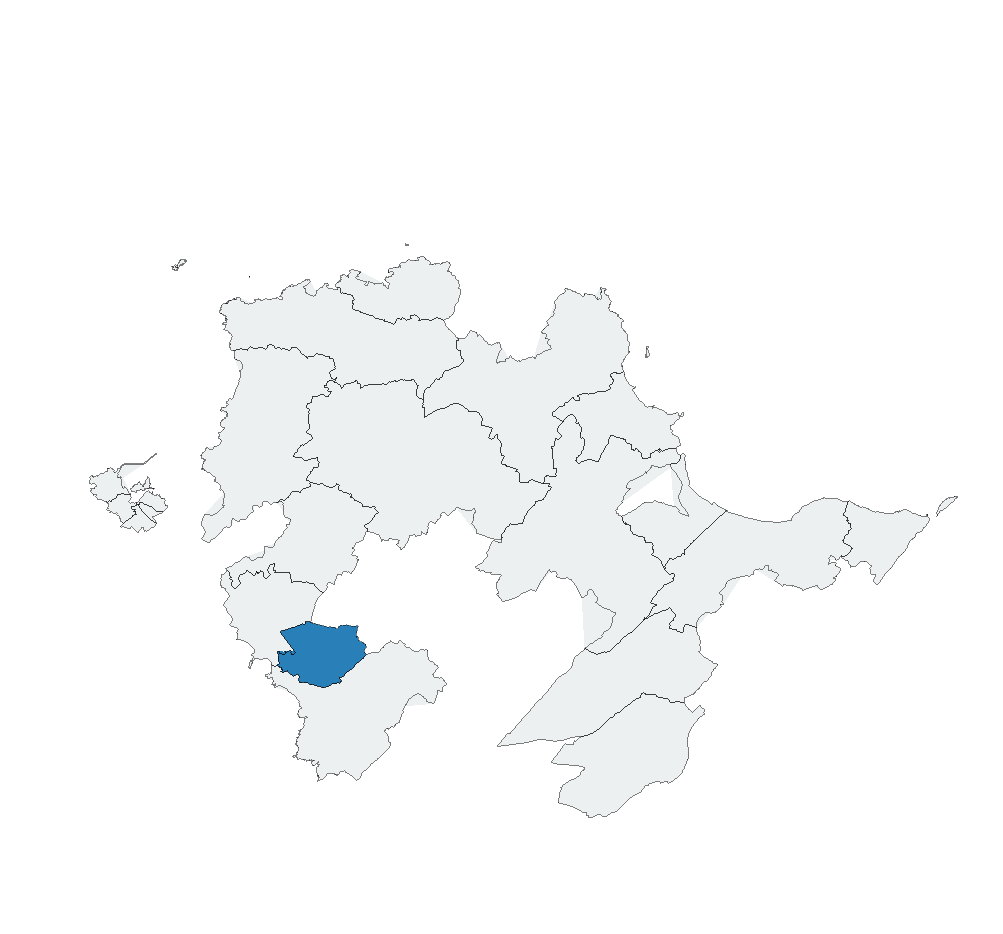
\includegraphics[width=1\linewidth]{images/ch6/loading/13}&
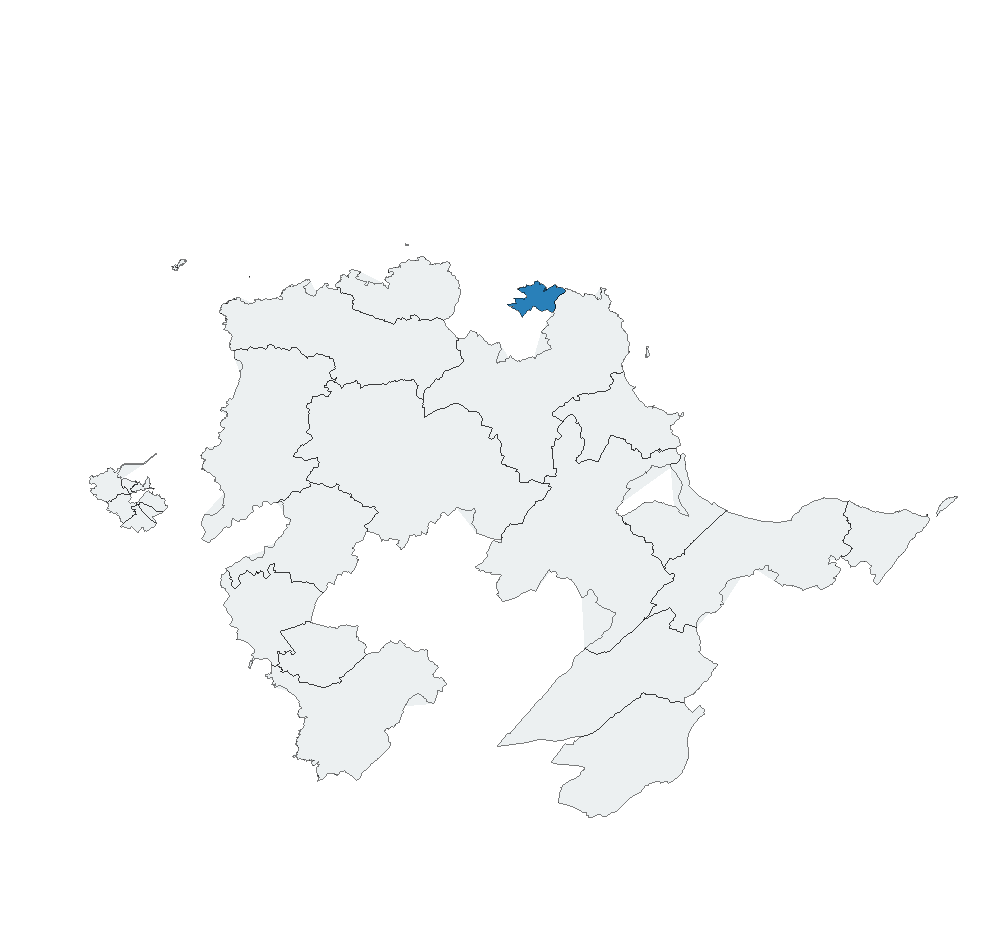
\includegraphics[width=1\linewidth]{images/ch6/loading/14}&
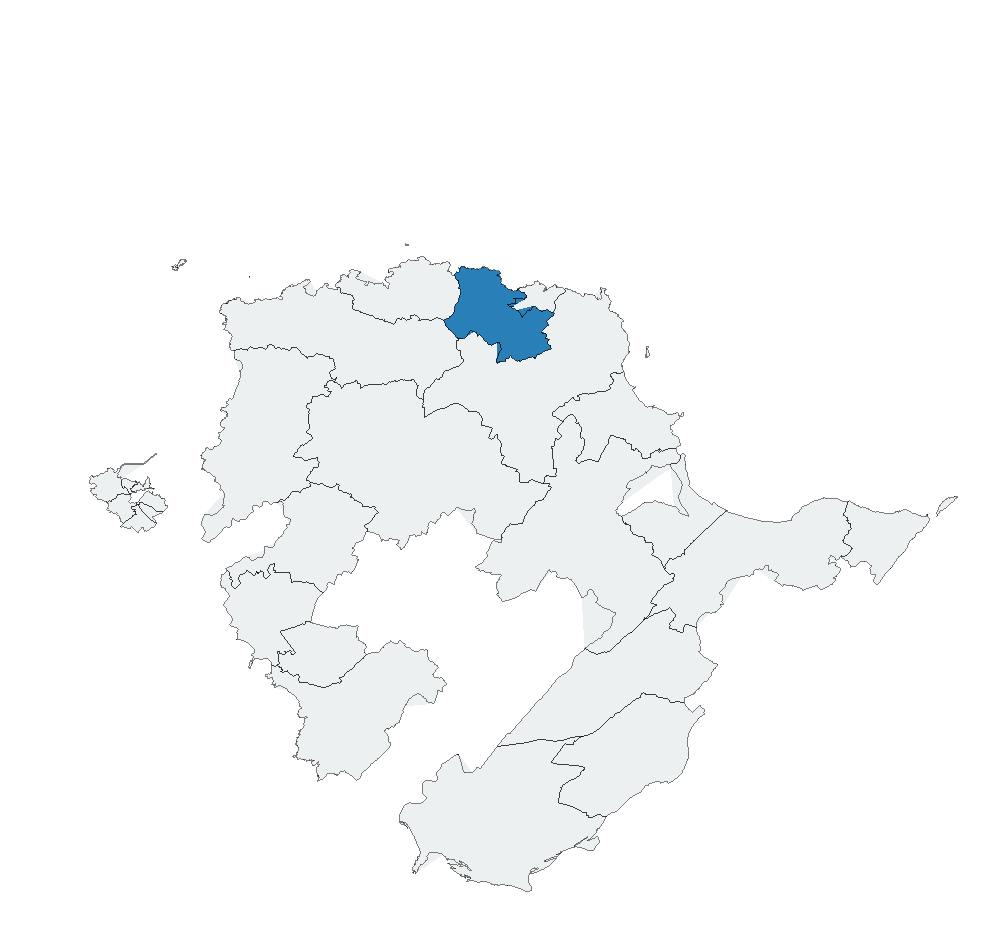
\includegraphics[width=1\linewidth]{images/ch6/loading/15}&
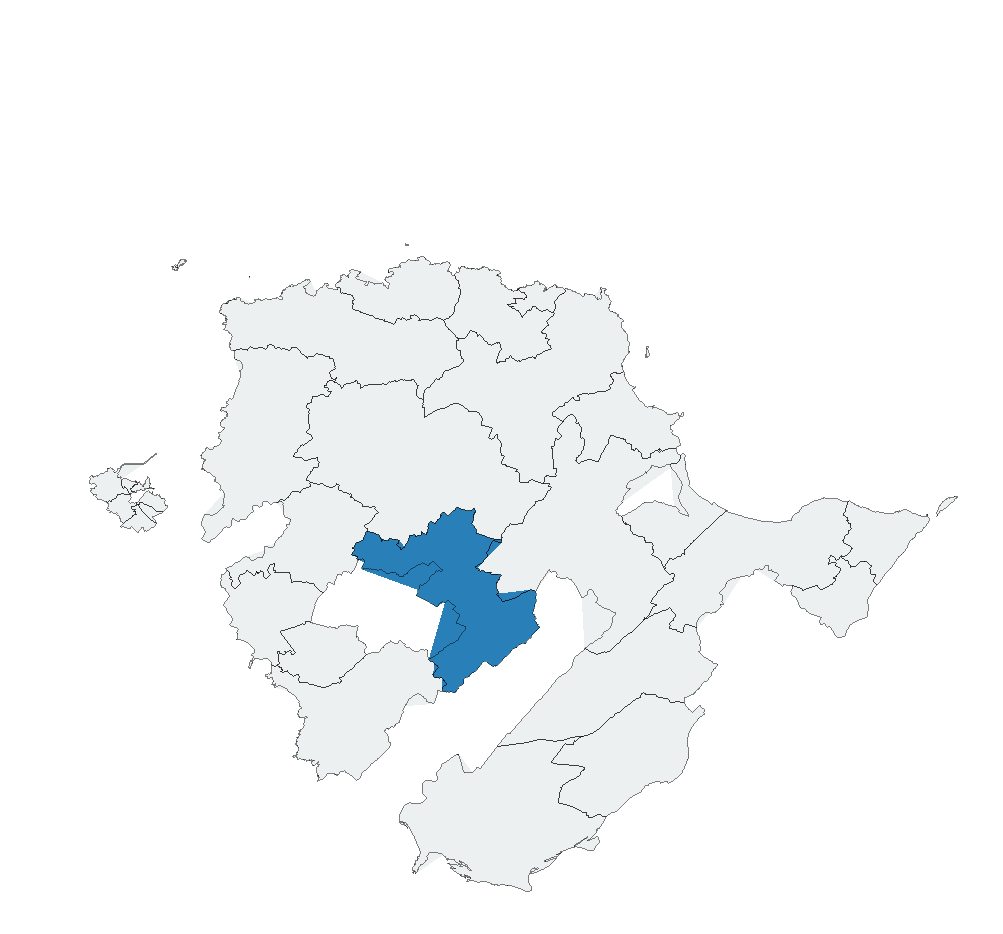
\includegraphics[width=1\linewidth]{images/ch6/loading/16} \\
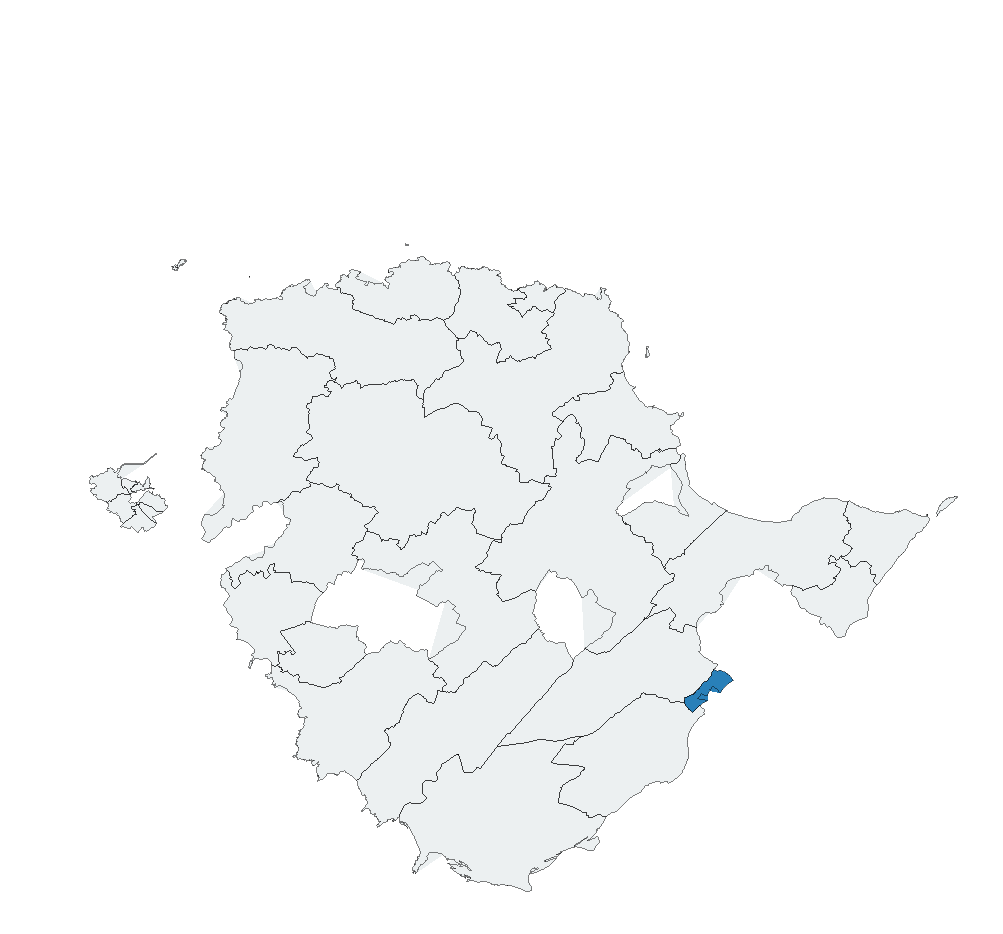
\includegraphics[width=1\linewidth]{images/ch6/loading/17}&
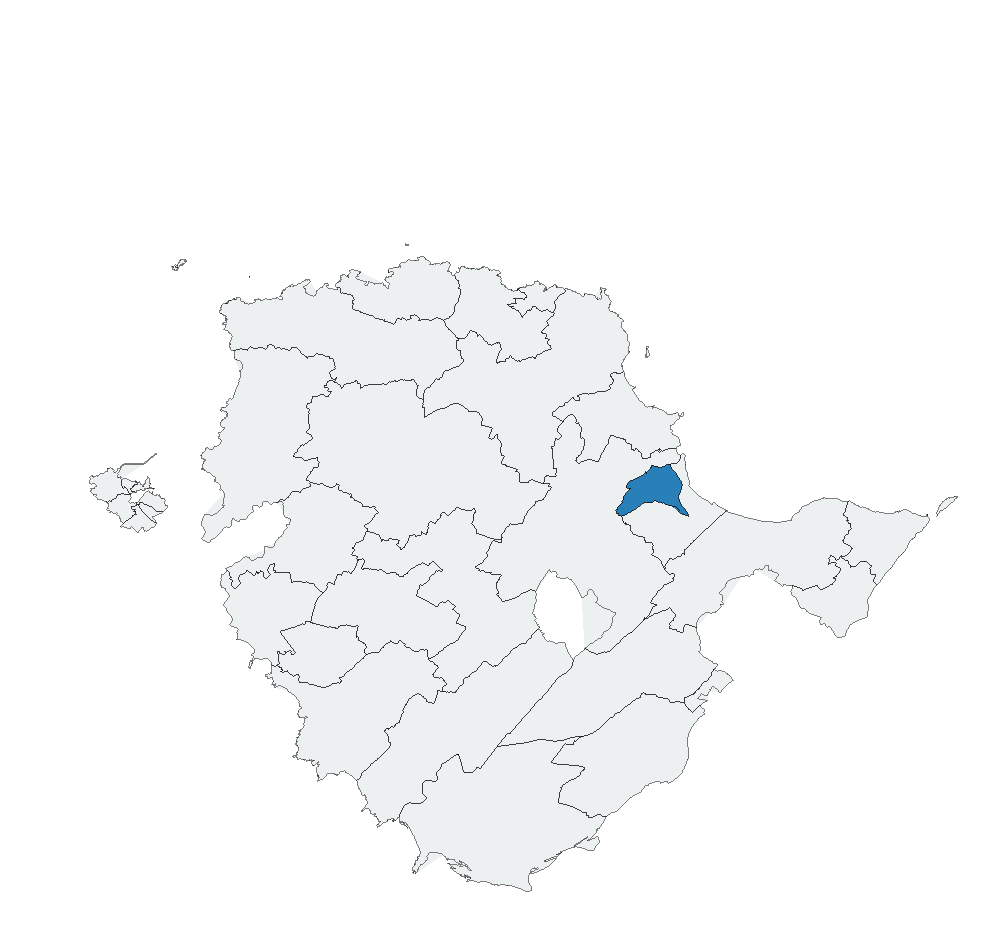
\includegraphics[width=1\linewidth]{images/ch6/loading/18}&
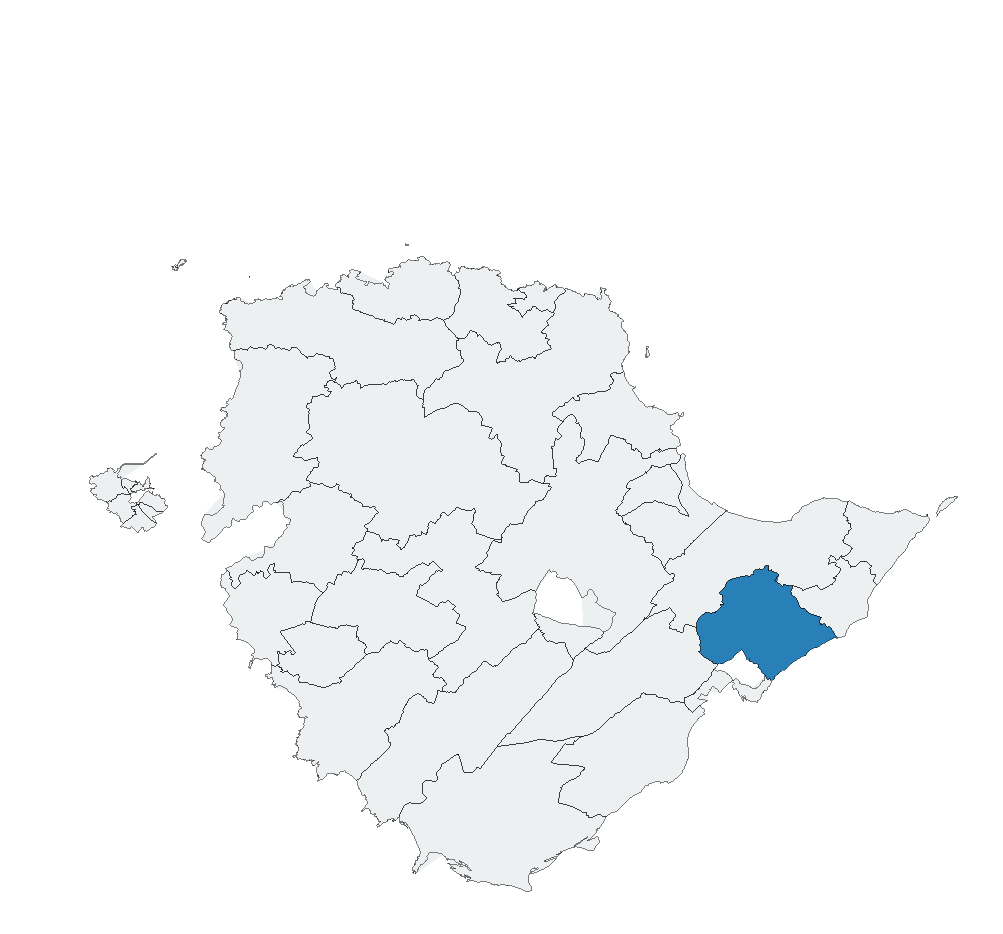
\includegraphics[width=1\linewidth]{images/ch6/loading/19}&
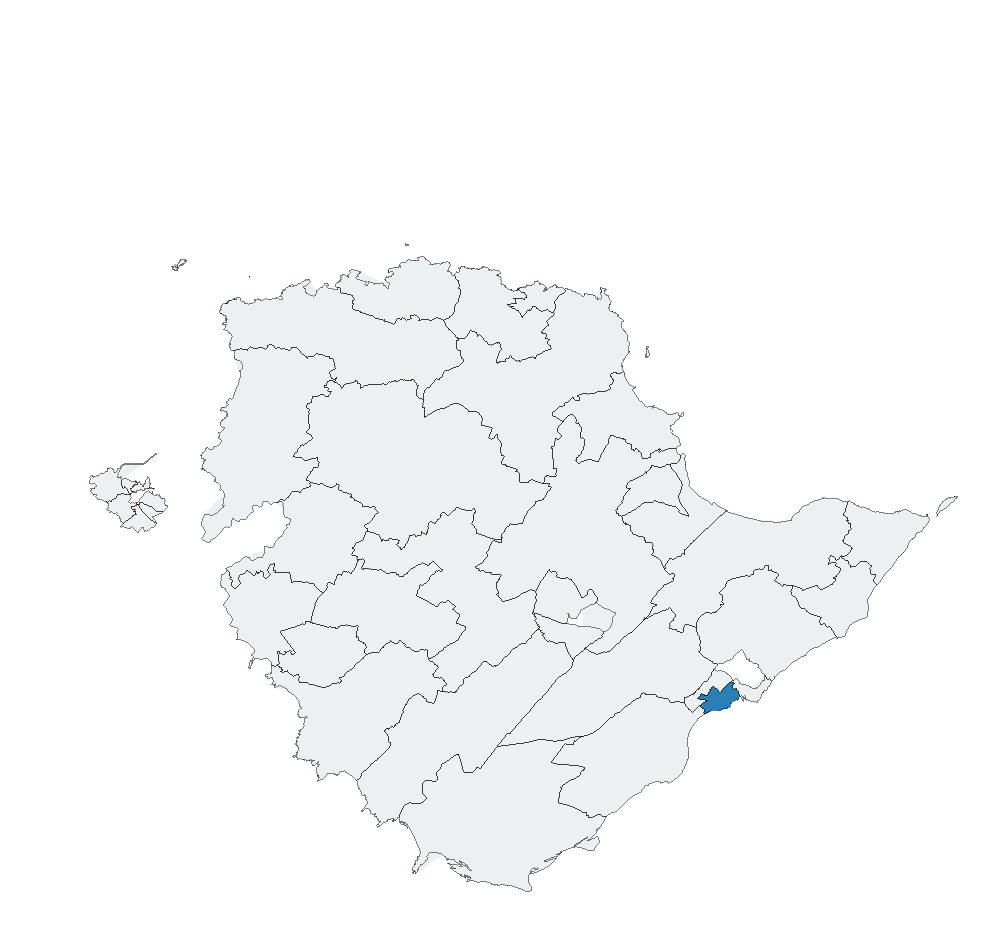
\includegraphics[width=1\linewidth]{images/ch6/loading/20} \\
%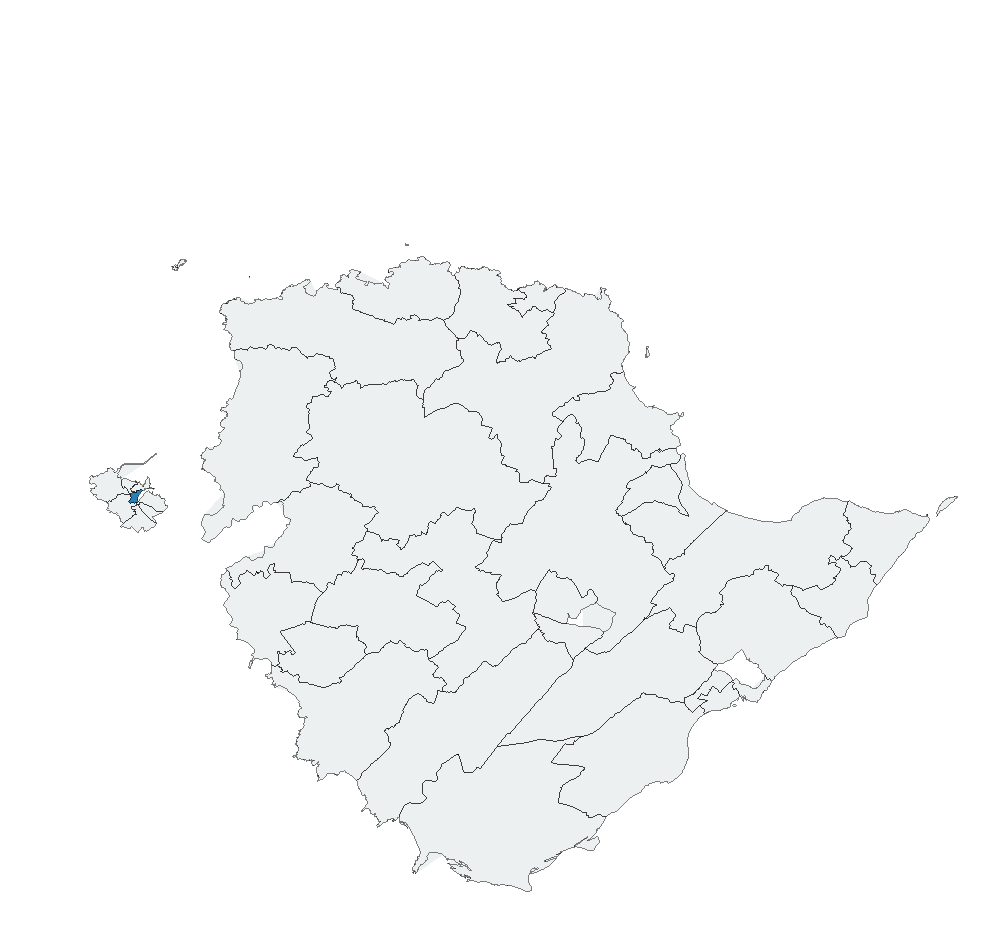
\includegraphics[width=1\linewidth]{images/ch6/loading/21}&
%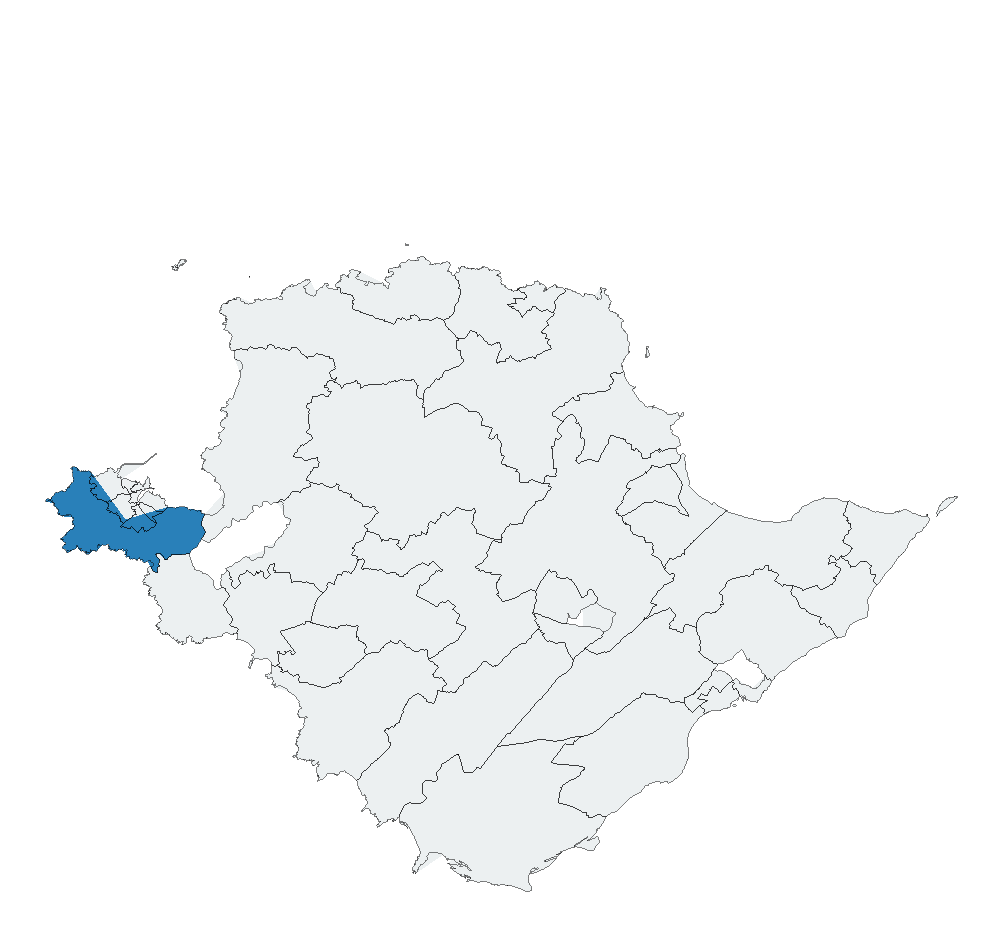
\includegraphics[width=1\linewidth]{images/ch6/loading/22}&
%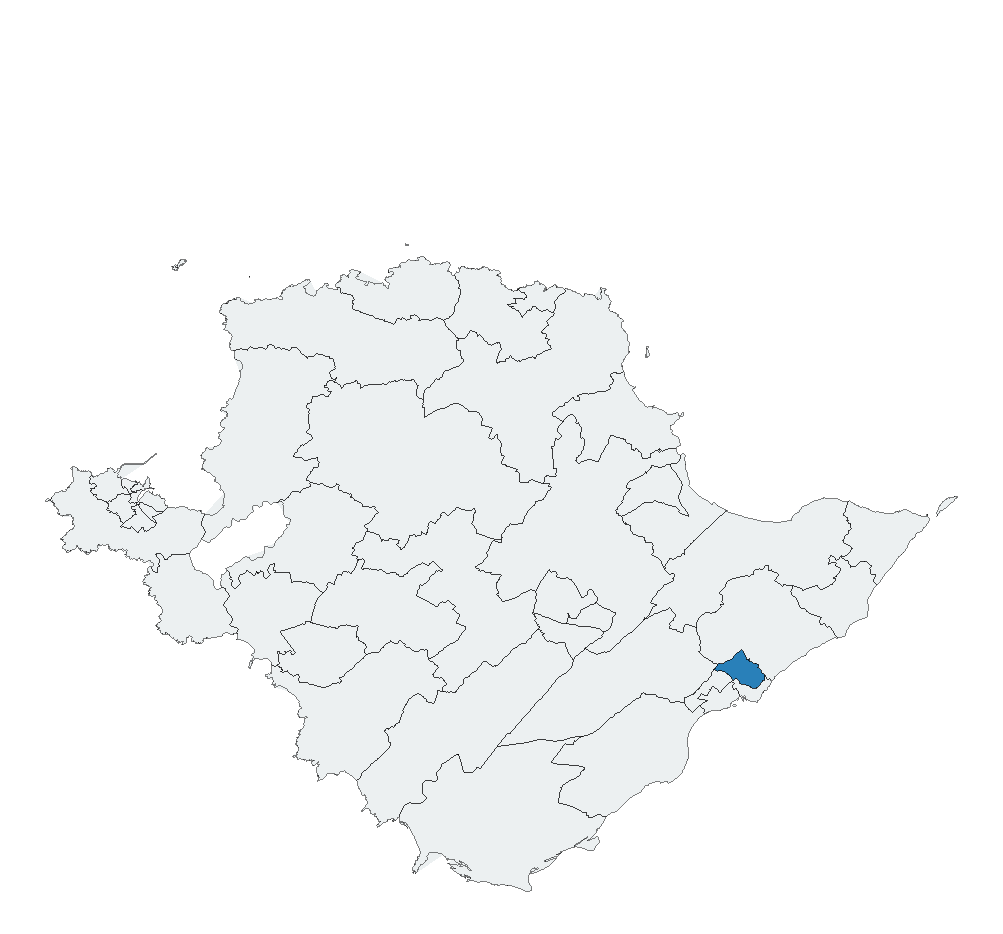
\includegraphics[width=1\linewidth]{images/ch6/loading/23}&
%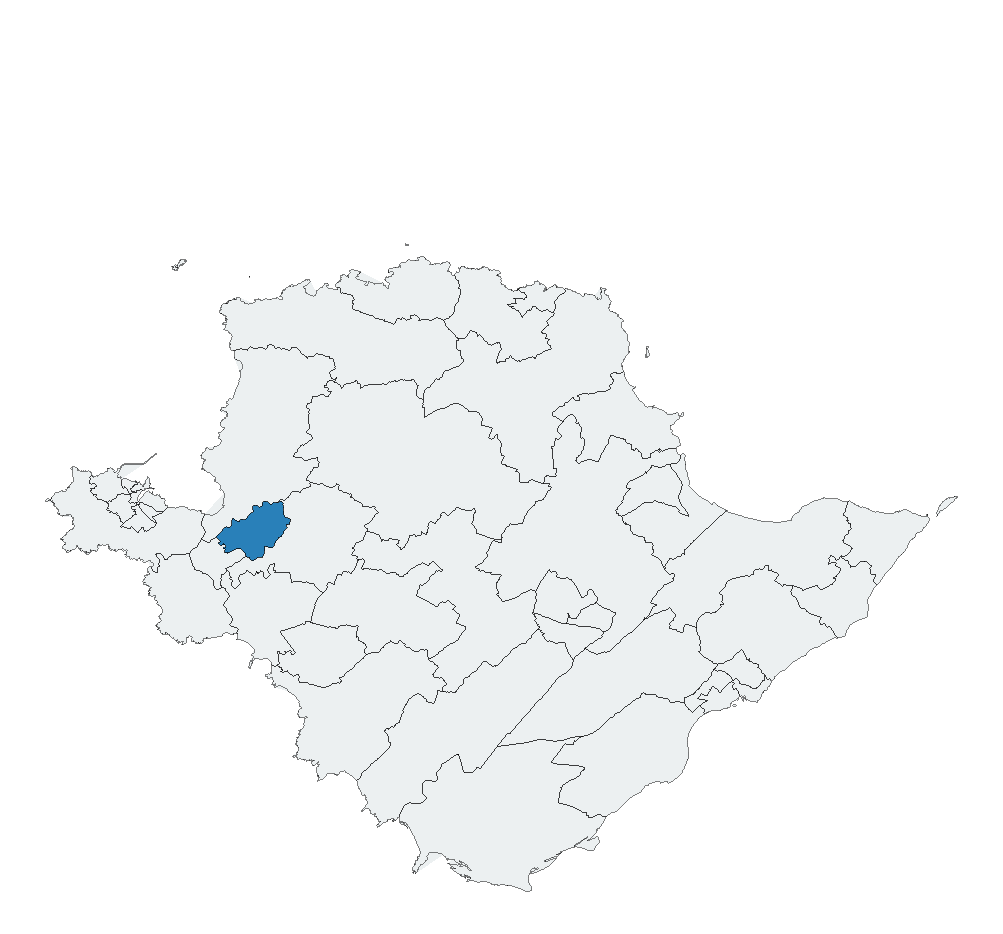
\includegraphics[width=1\linewidth]{images/ch6/loading/24} \\ %24
\end{tabularx}
\caption{A matrix depicting time slices of the temporal debug visualization for geospatial debug loading. The blue presents the last loaded polygon, whilst the grey represent polygons that have already been loaded. The file represents a test data set taken from the LSOA's of Wales, specifically the contiguous mainland of Anglesy \cite{wales}.} \label{fig:loadingMatrix}
\end{figure}

\begin{figure}
\begin{tabularx}{1\textwidth}{XXXX}
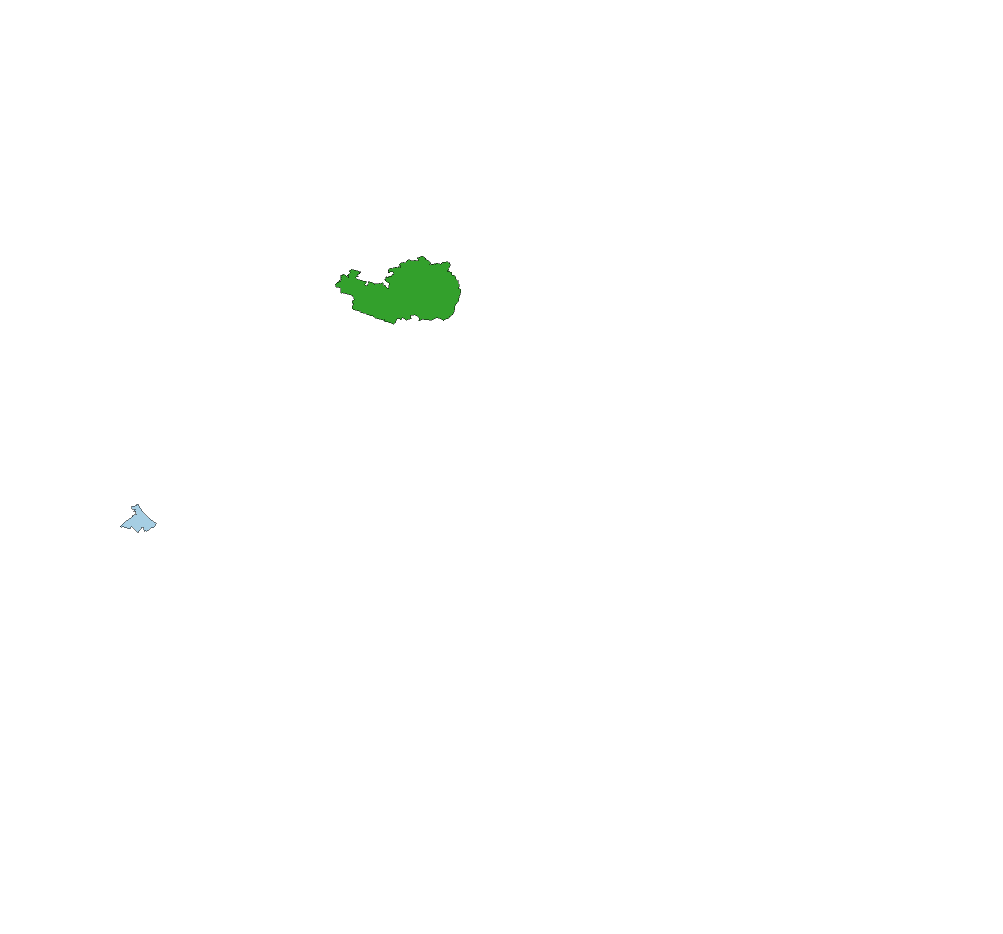
\includegraphics[width=1\linewidth]{images/ch6/contig/01}&
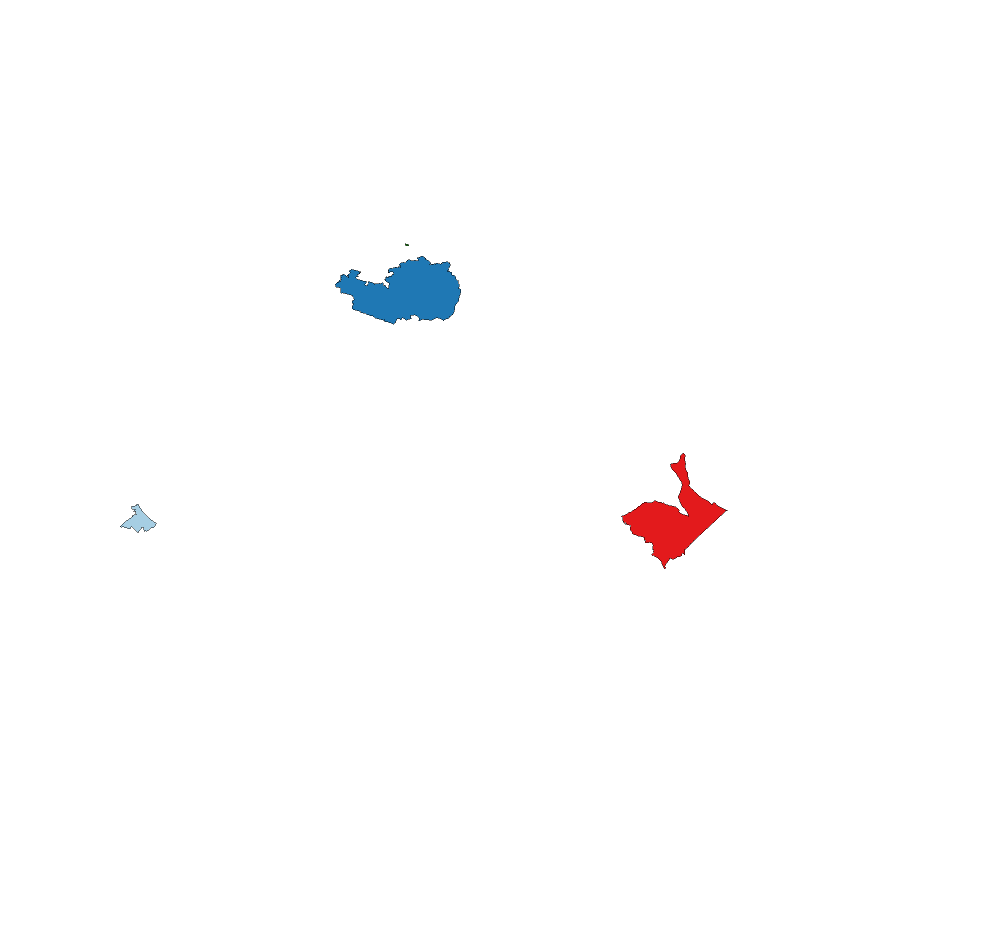
\includegraphics[width=1\linewidth]{images/ch6/contig/02}&
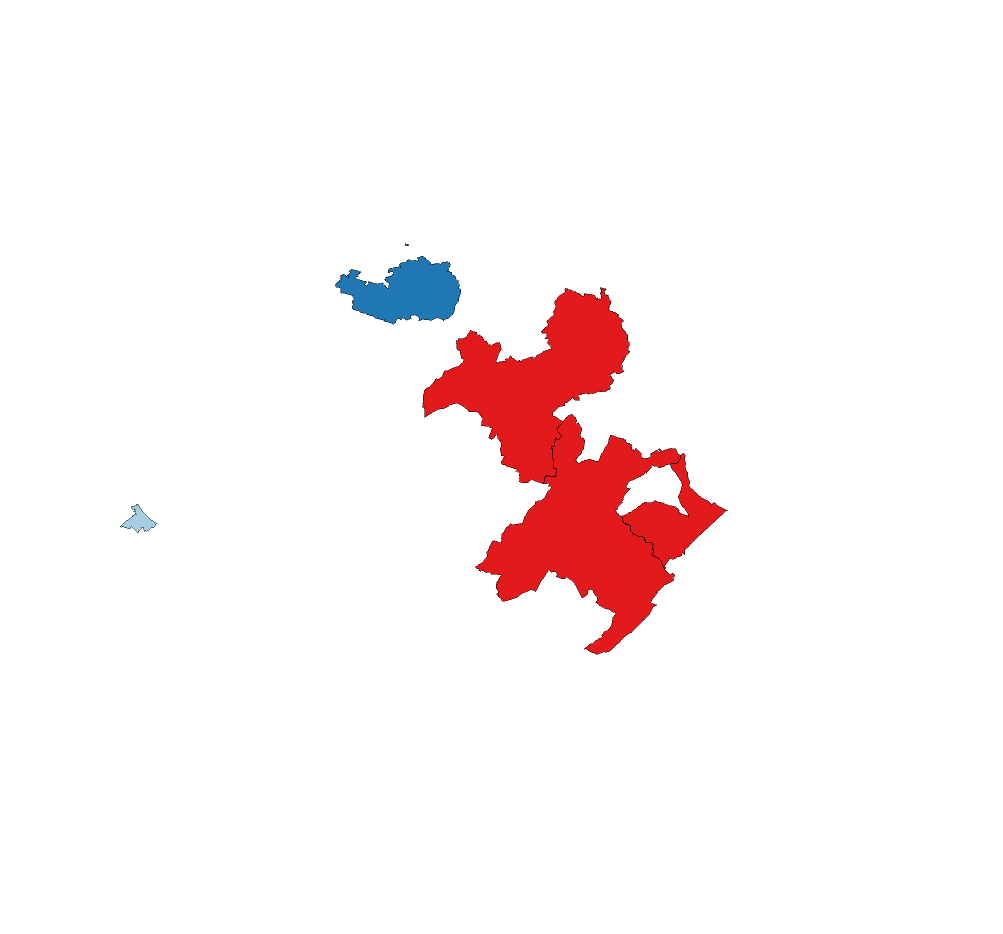
\includegraphics[width=1\linewidth]{images/ch6/contig/03}&
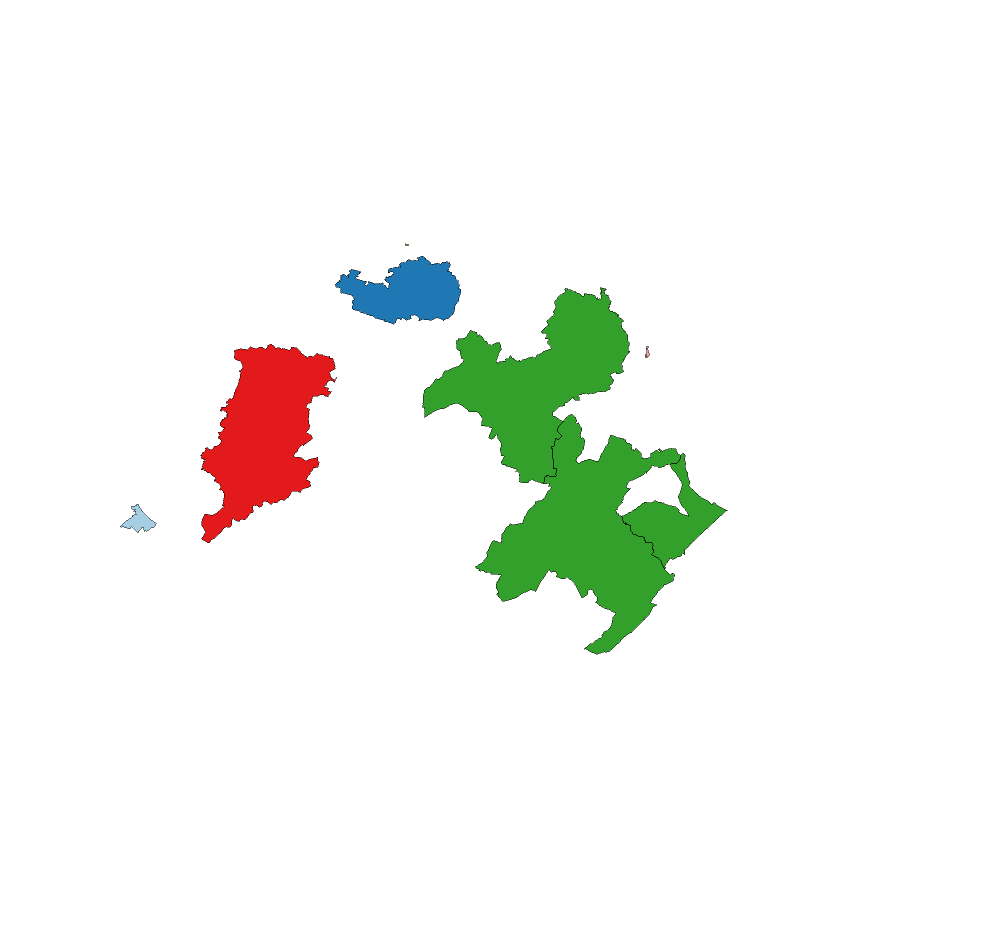
\includegraphics[width=1\linewidth]{images/ch6/contig/04} \\
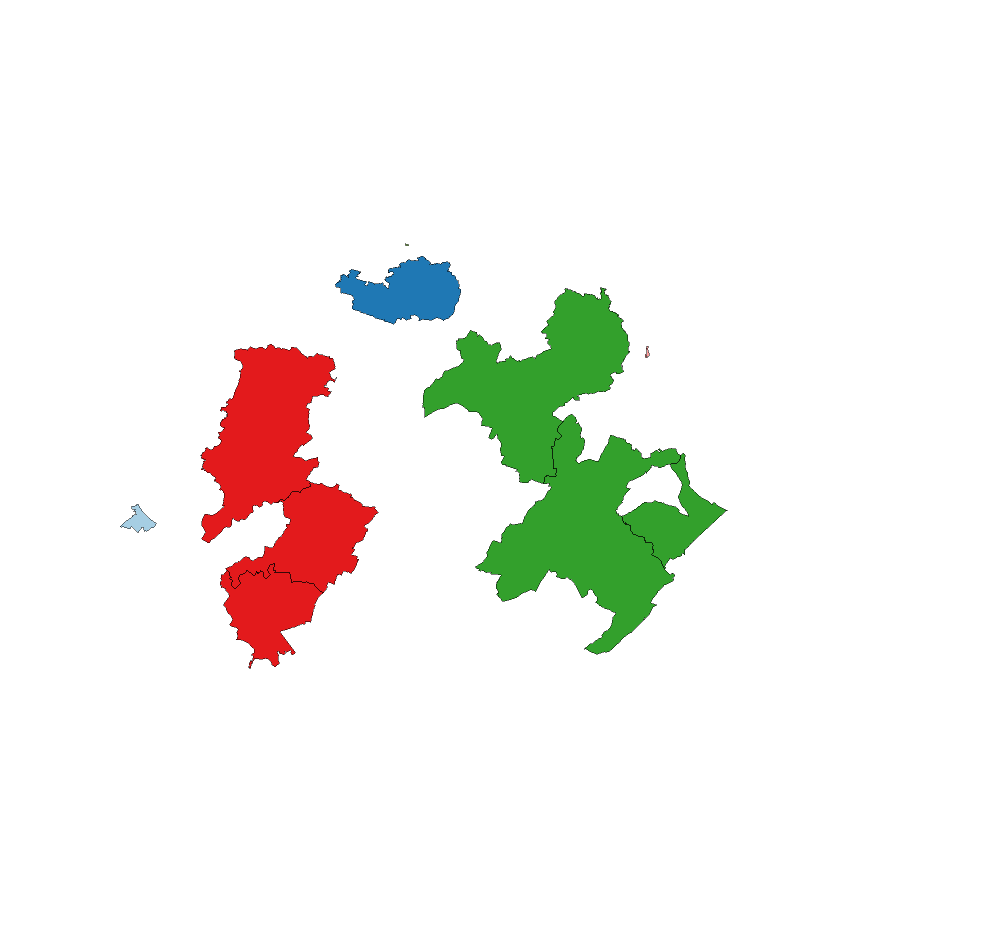
\includegraphics[width=1\linewidth]{images/ch6/contig/05}&
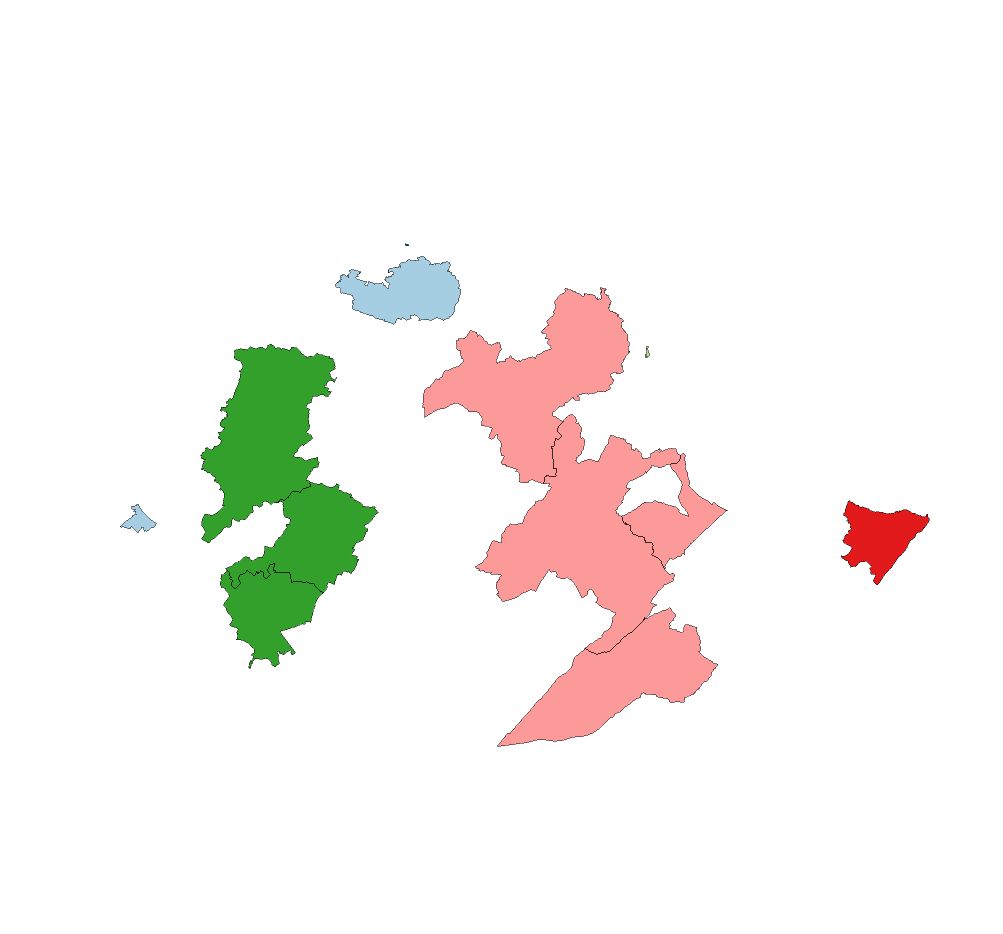
\includegraphics[width=1\linewidth]{images/ch6/contig/06}&
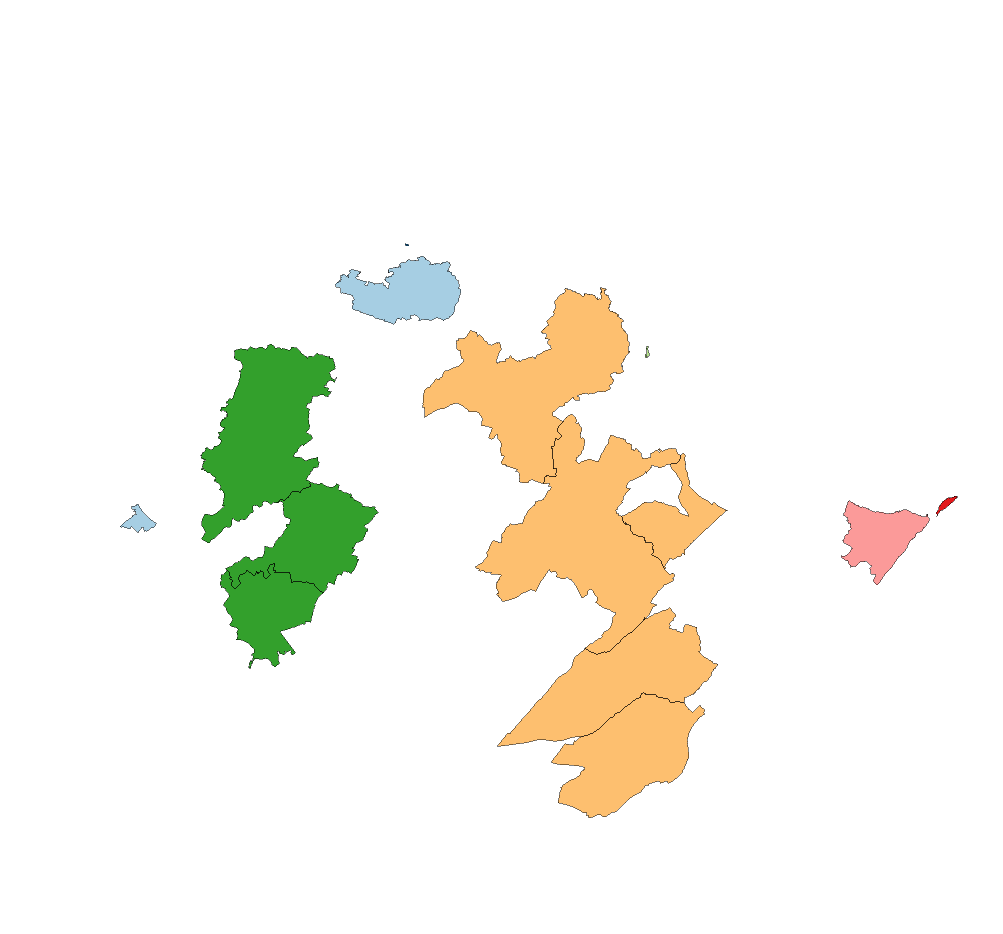
\includegraphics[width=1\linewidth]{images/ch6/contig/07}&
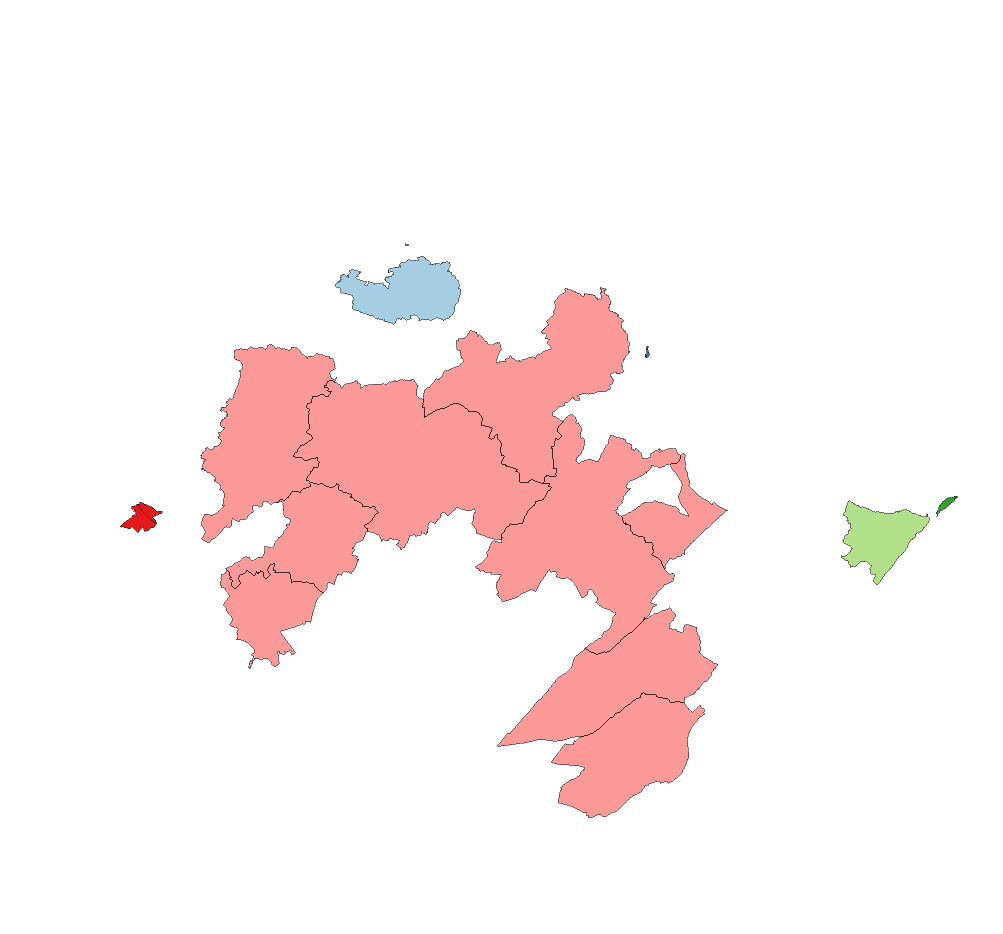
\includegraphics[width=1\linewidth]{images/ch6/contig/08} \\
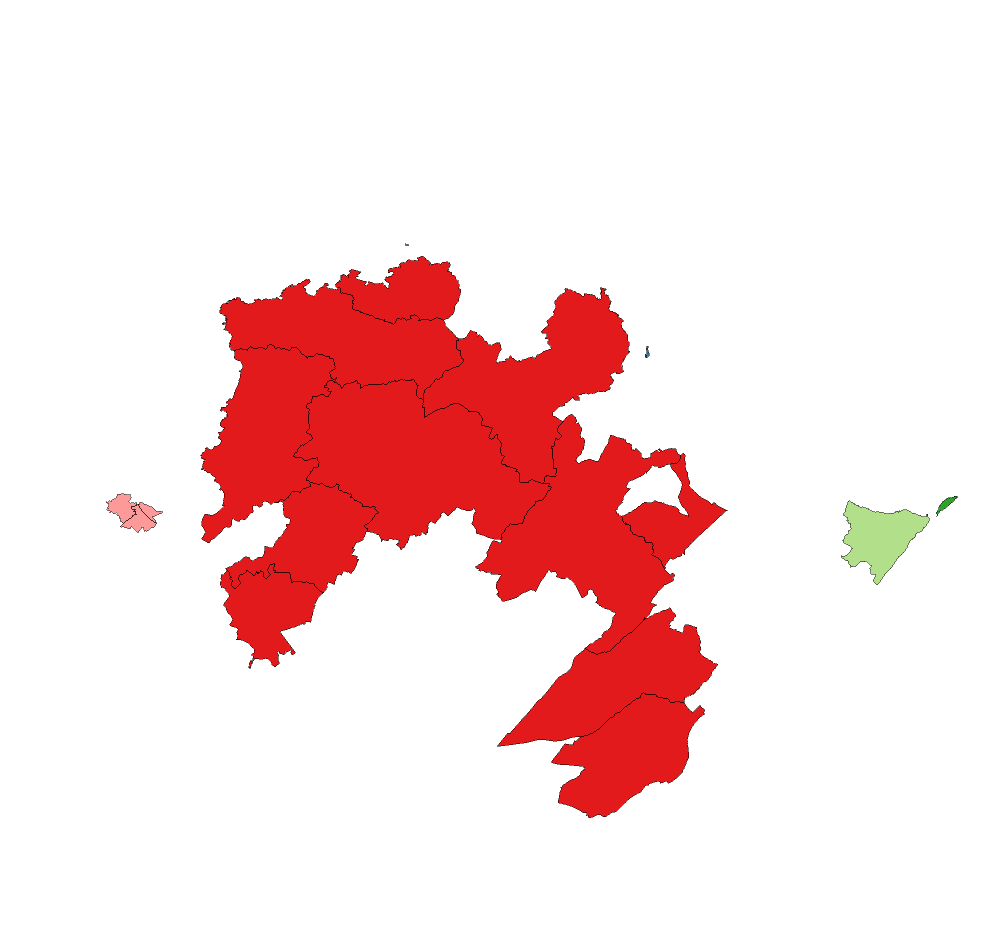
\includegraphics[width=1\linewidth]{images/ch6/contig/09}&
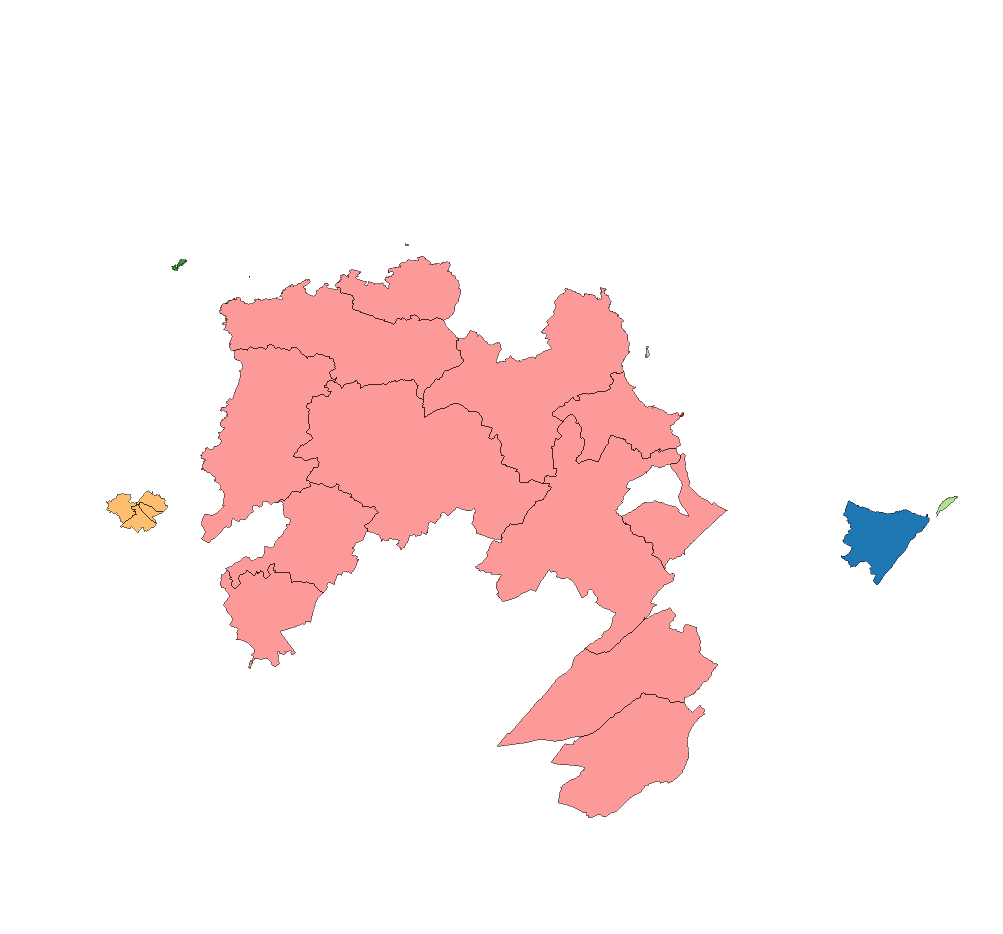
\includegraphics[width=1\linewidth]{images/ch6/contig/10}&
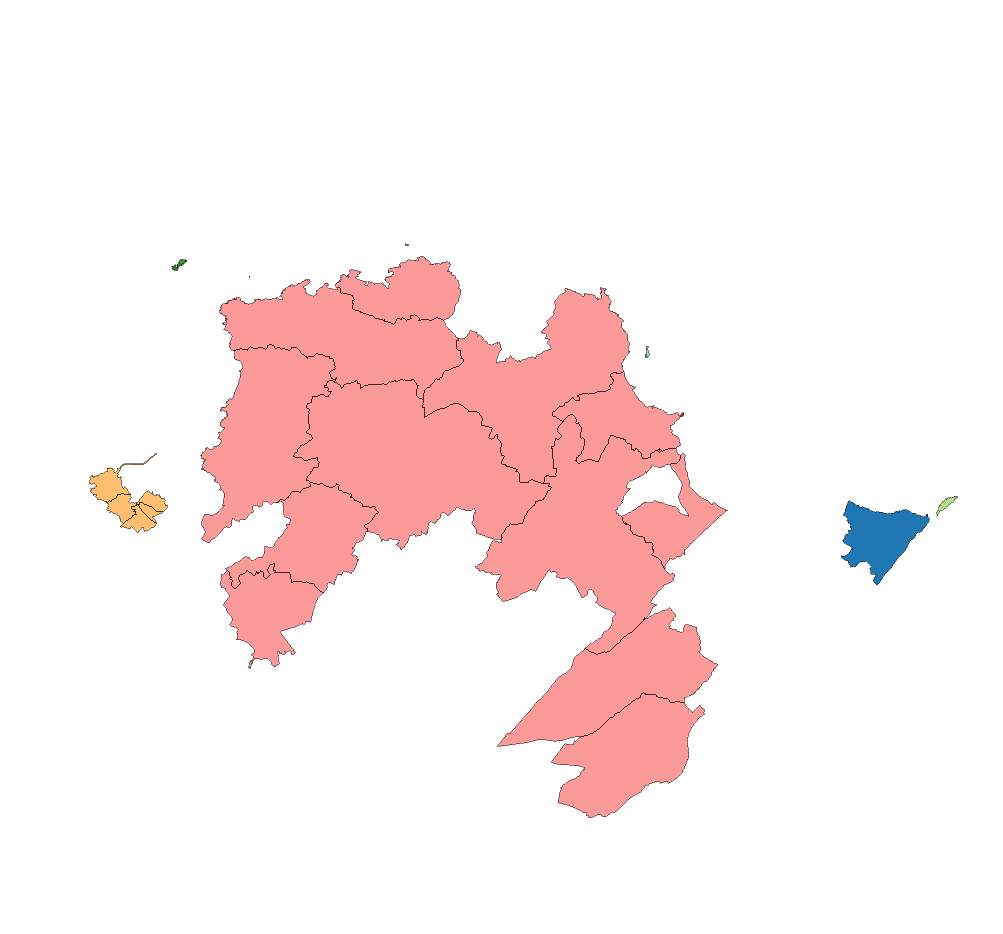
\includegraphics[width=1\linewidth]{images/ch6/contig/11}&
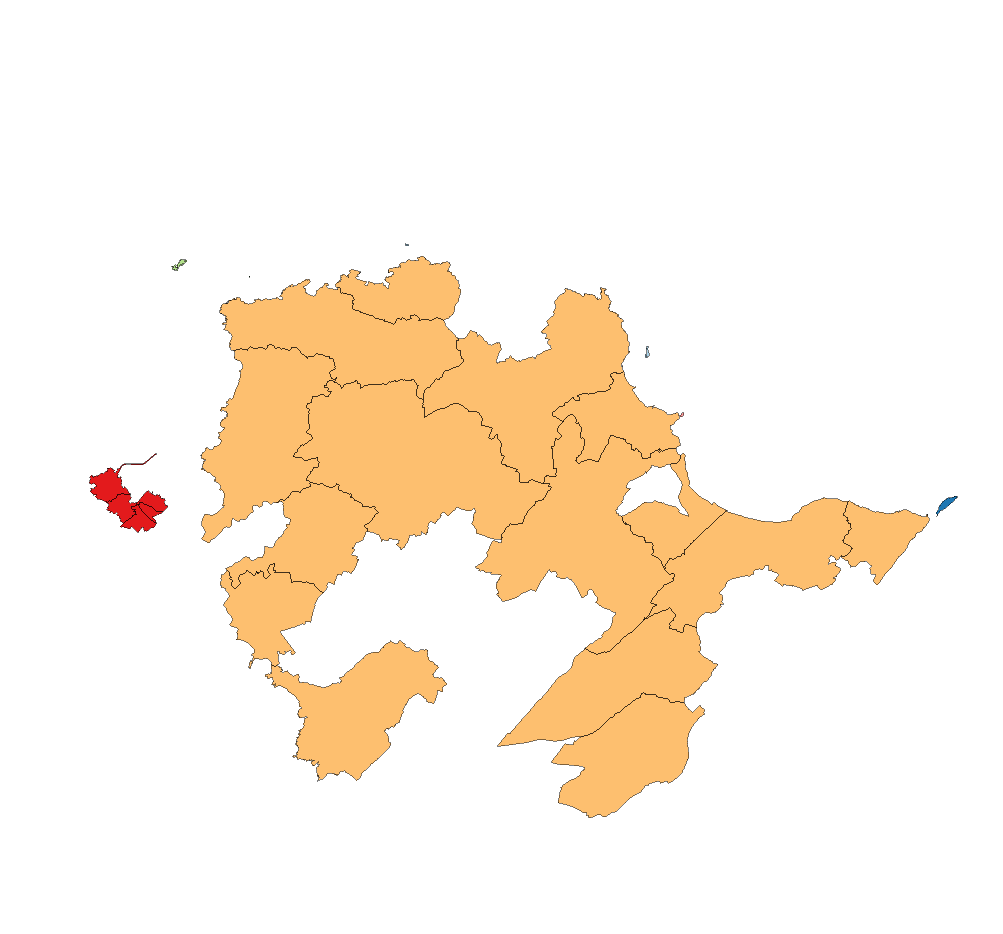
\includegraphics[width=1\linewidth]{images/ch6/contig/12} \\
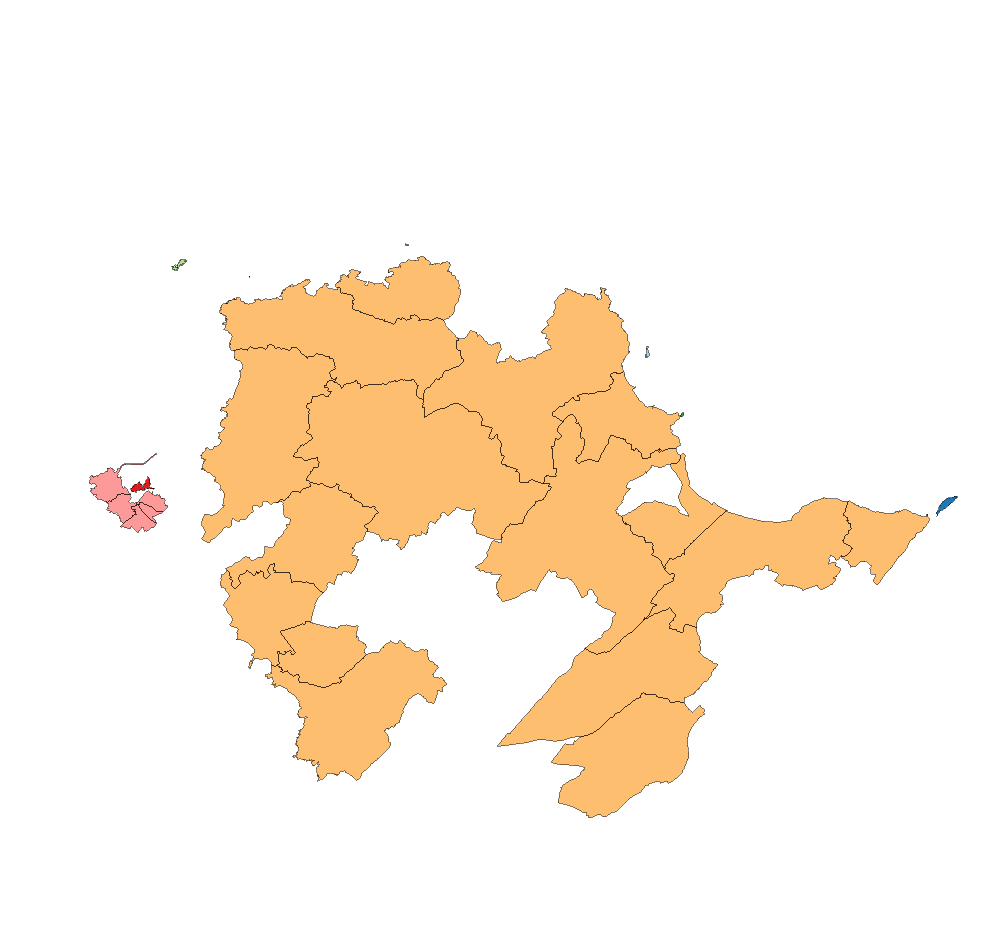
\includegraphics[width=1\linewidth]{images/ch6/contig/13}&
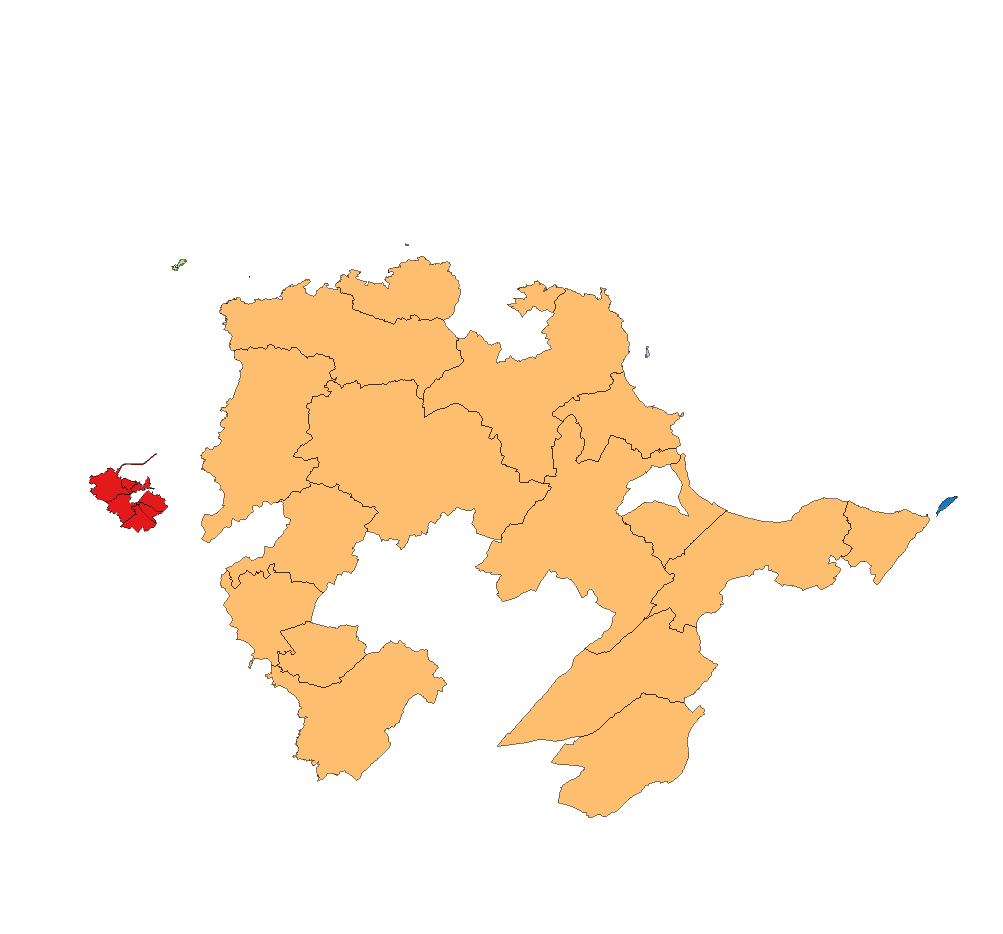
\includegraphics[width=1\linewidth]{images/ch6/contig/14}&
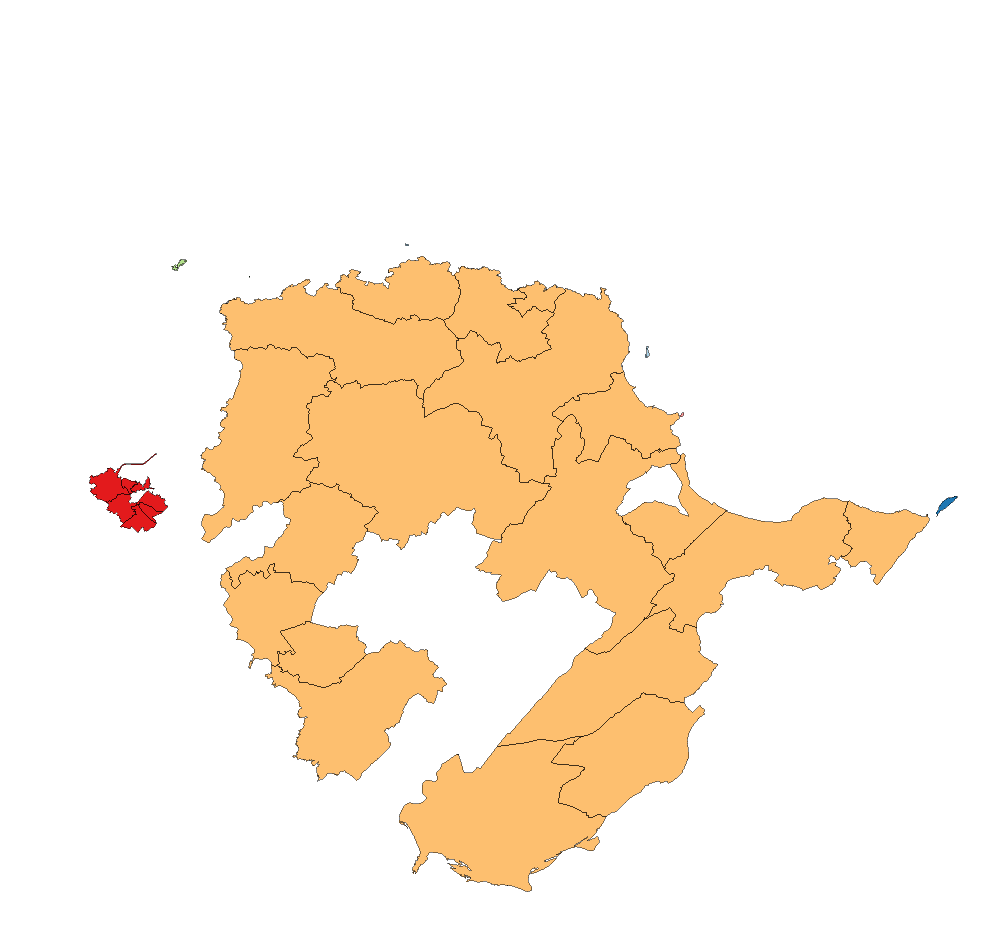
\includegraphics[width=1\linewidth]{images/ch6/contig/15}&
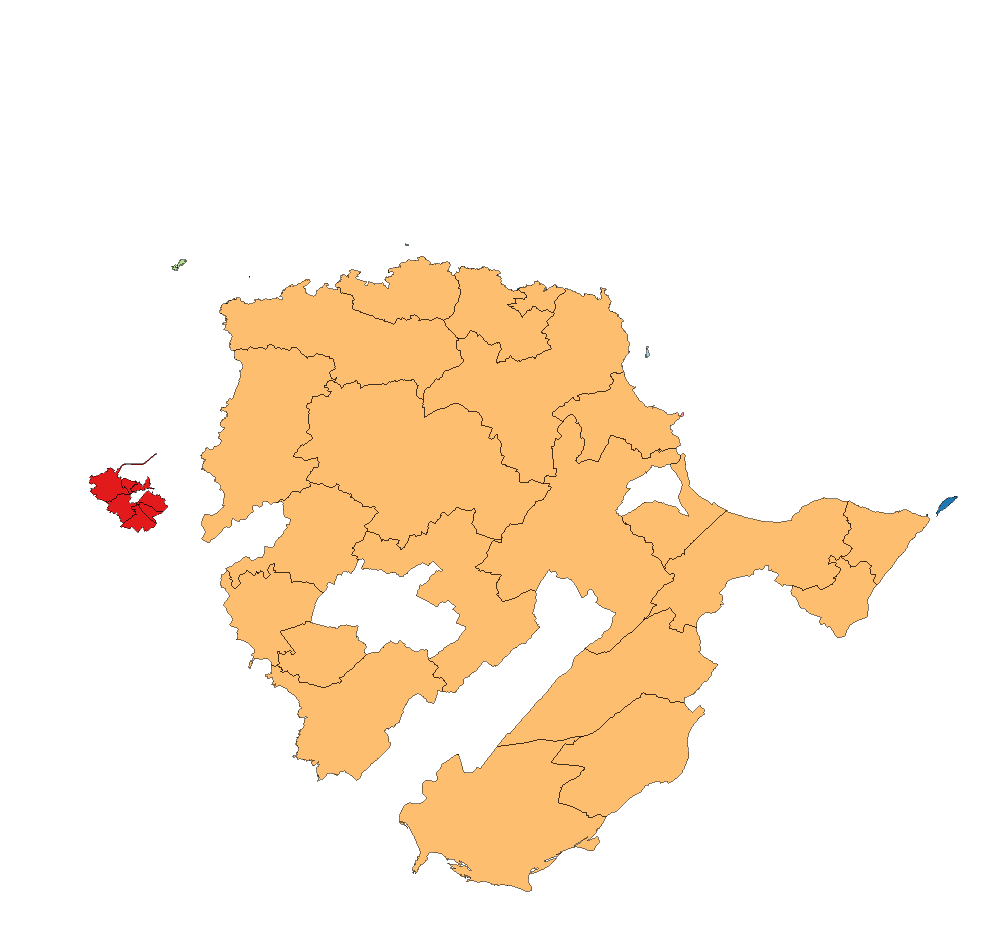
\includegraphics[width=1\linewidth]{images/ch6/contig/16} \\
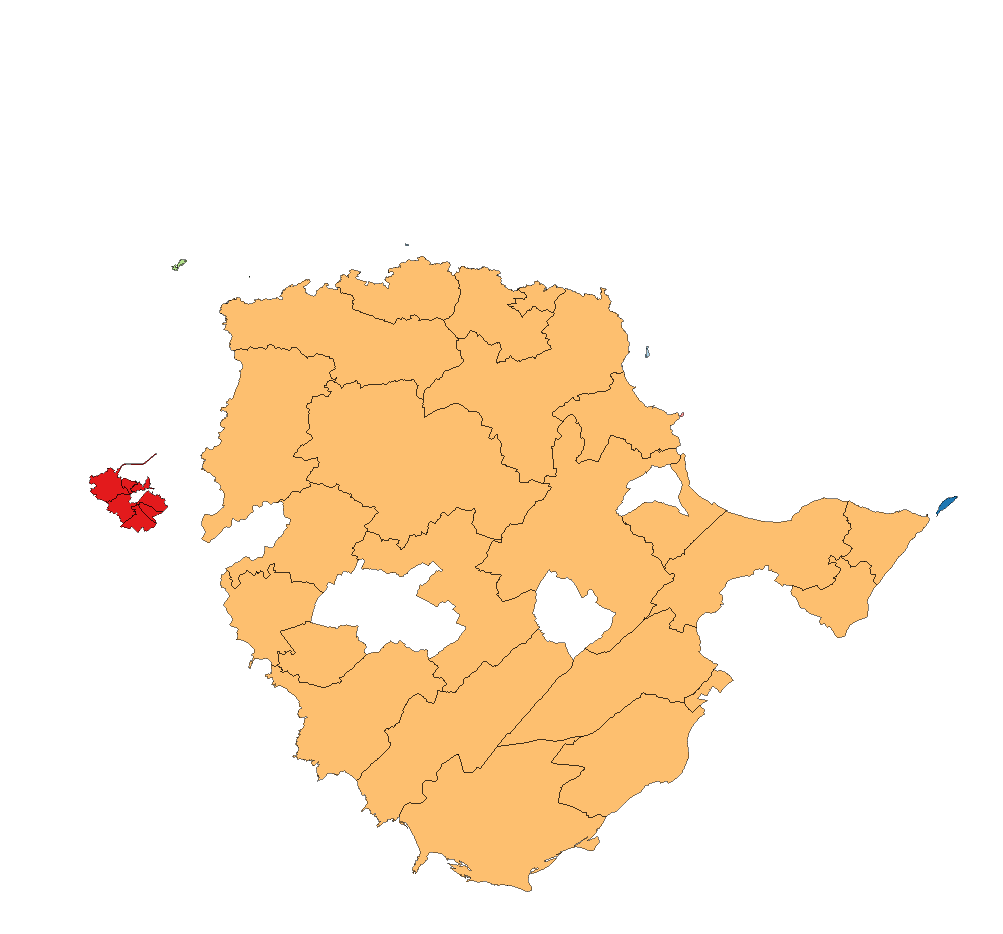
\includegraphics[width=1\linewidth]{images/ch6/contig/17}&
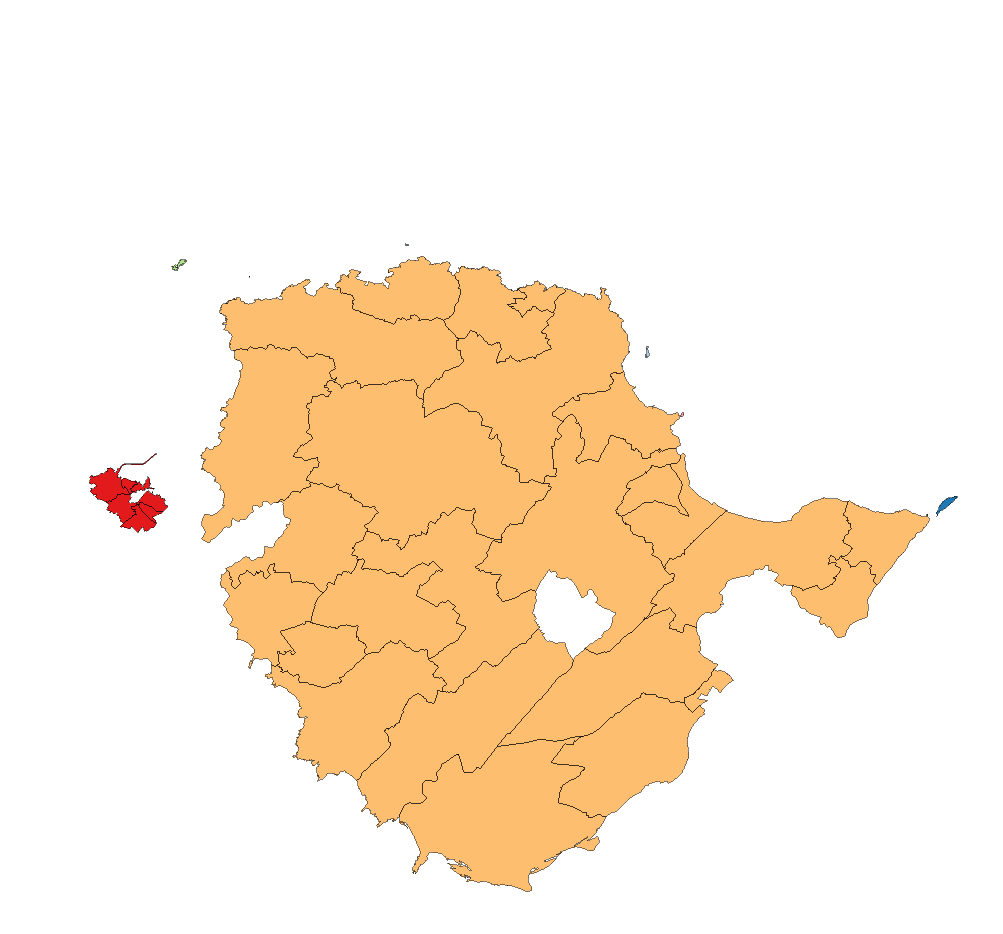
\includegraphics[width=1\linewidth]{images/ch6/contig/18}&
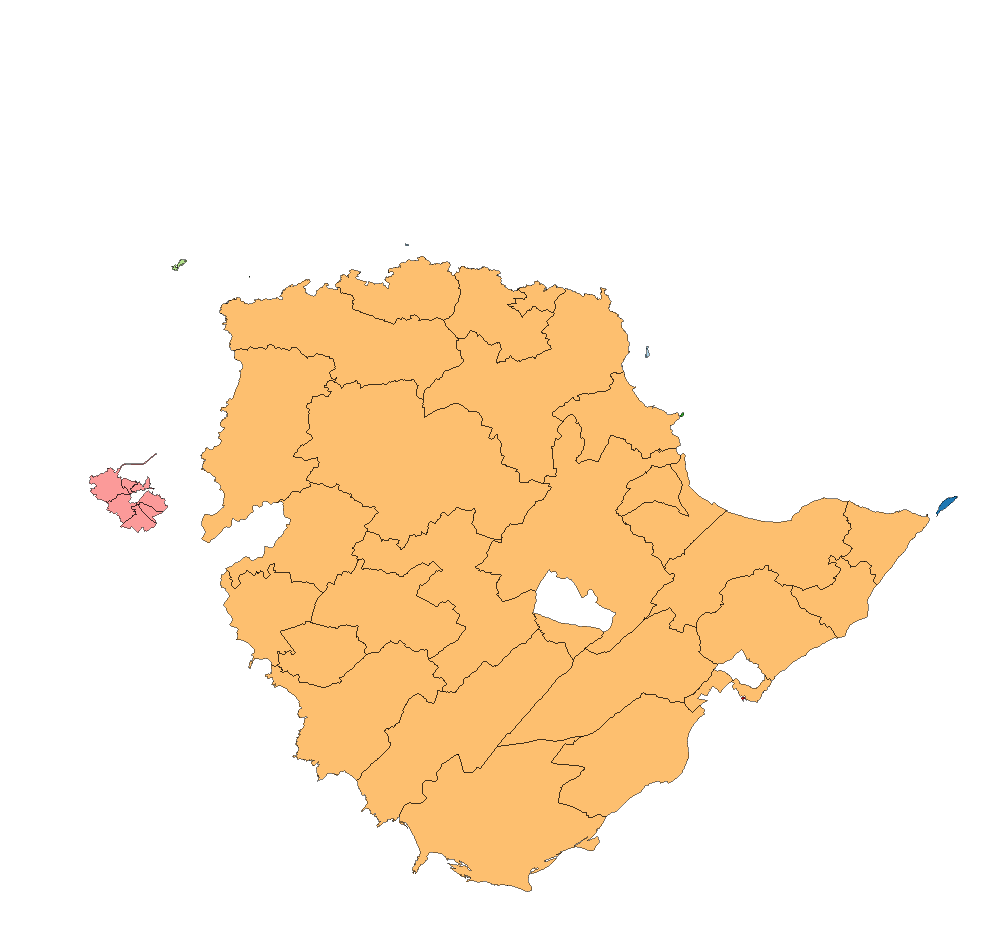
\includegraphics[width=1\linewidth]{images/ch6/contig/19}&
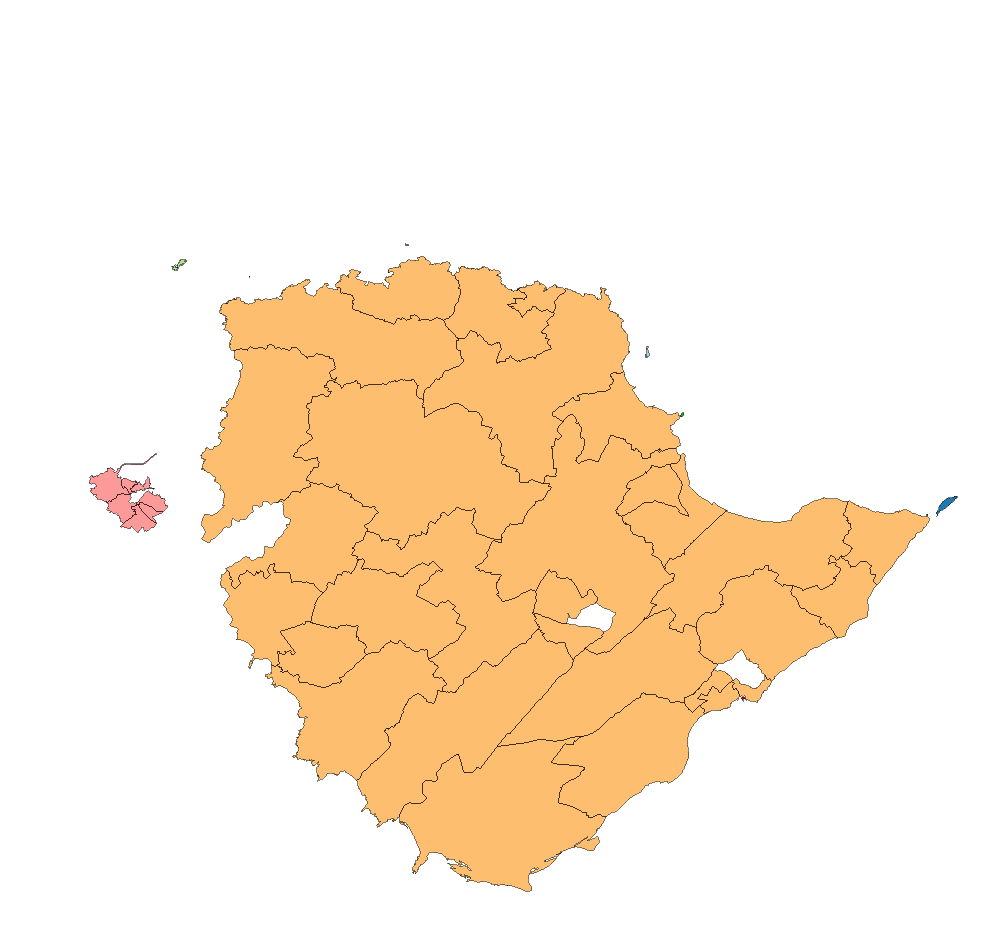
\includegraphics[width=1\linewidth]{images/ch6/contig/20} \\
%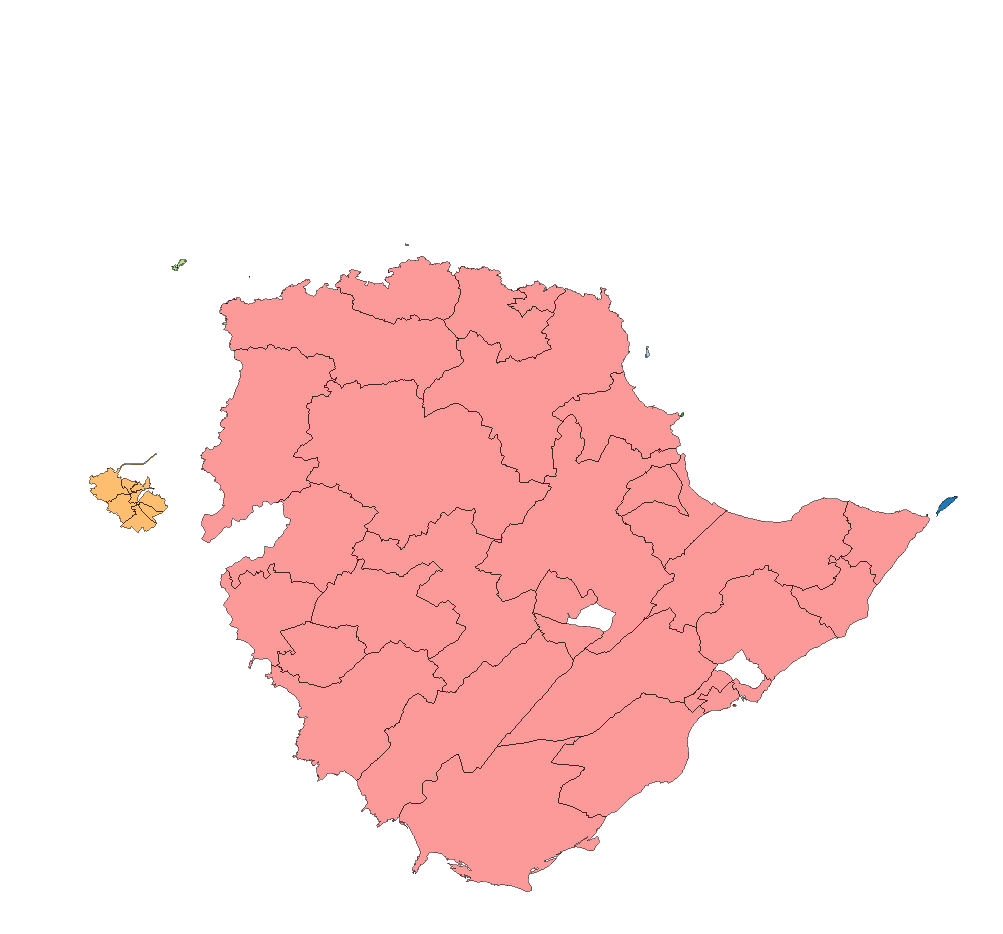
\includegraphics[width=1\linewidth]{images/ch6/contig/21}&
%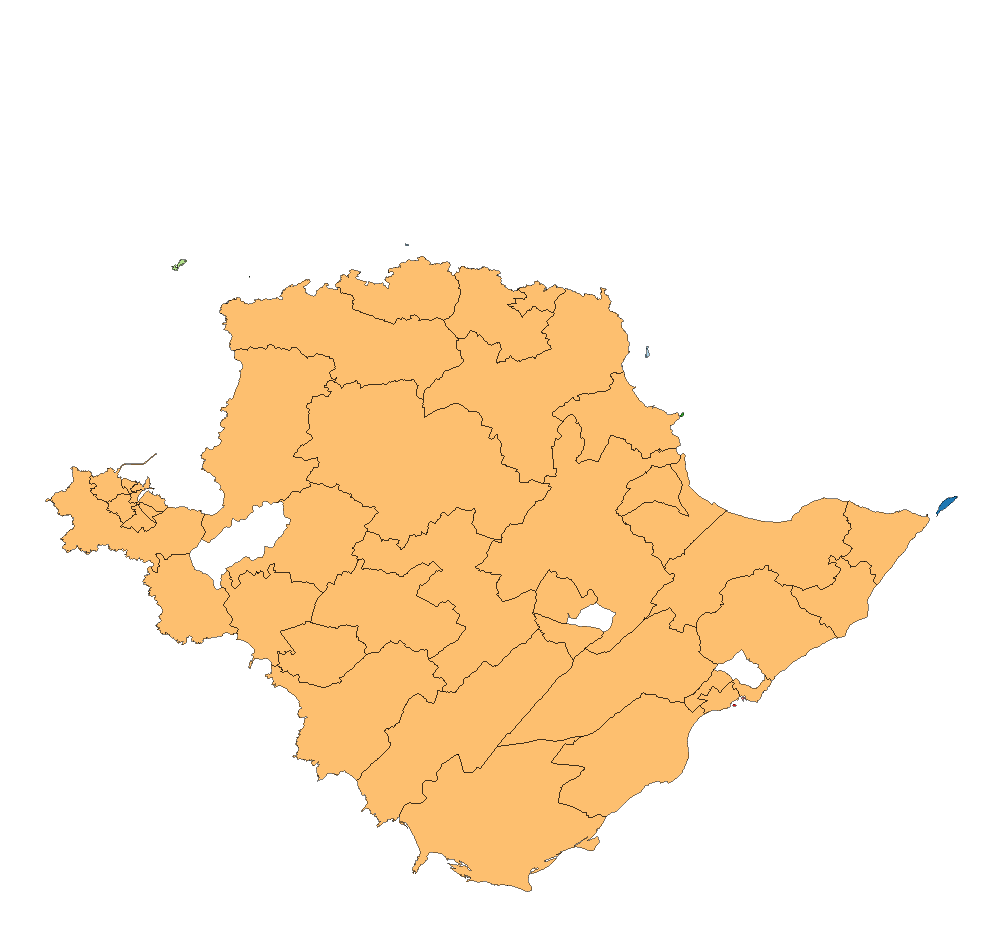
\includegraphics[width=1\linewidth]{images/ch6/contig/22}&
%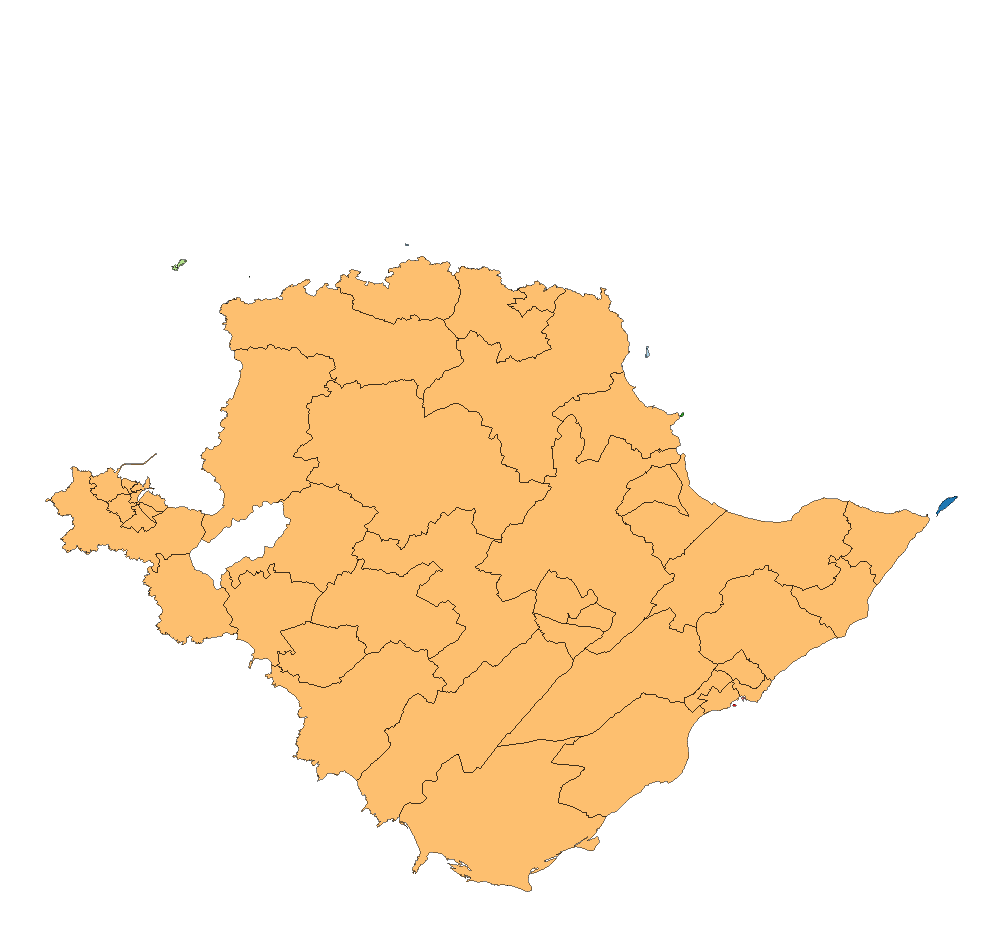
\includegraphics[width=1\linewidth]{images/ch6/contig/23}&
%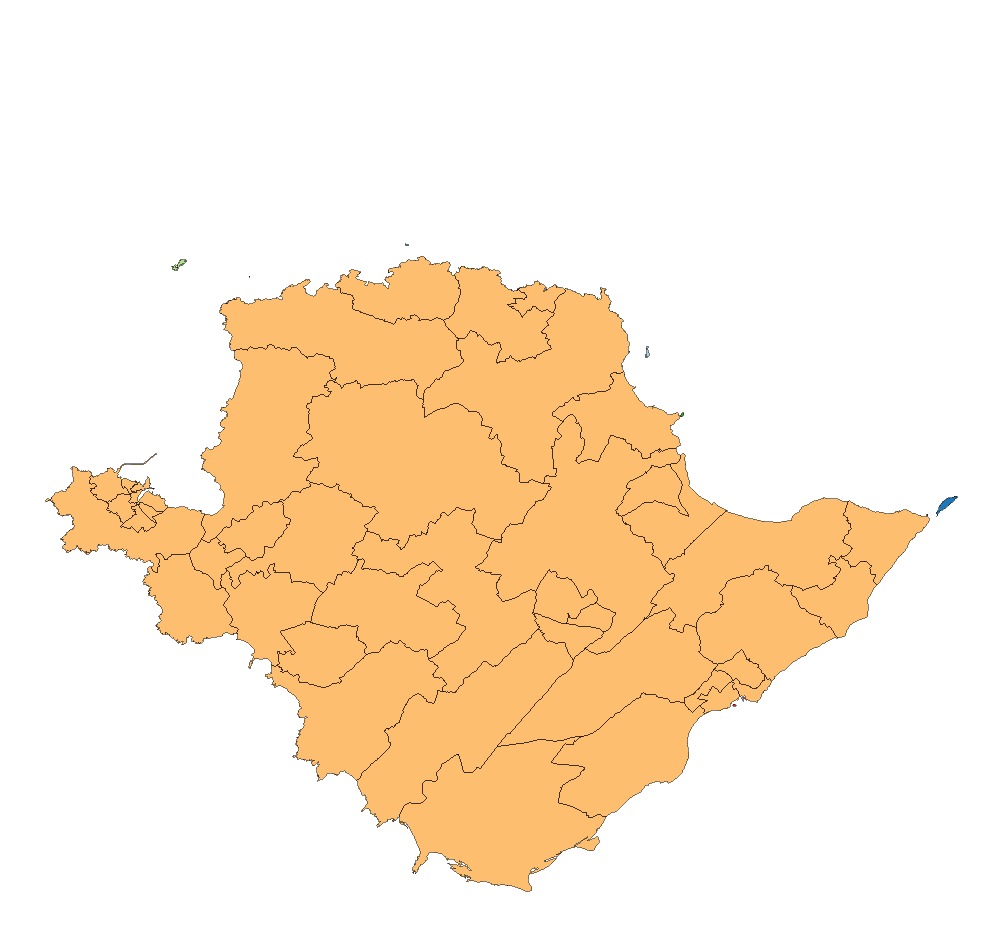
\includegraphics[width=1\linewidth]{images/ch6/contig/24} \\ %24
\end{tabularx}
\caption{A matrix depicting processing steps of the intermediate debug visualization for contiguity debugging. Each color rerpresents a contiguous region. The color considers the number of contiguous regions, and sets the last updated contiguous region to the most recent color. Test data set is relative to Figure \ref{fig:loadingMatrix} for comparison. The file represents a test data set taken from the LSOA's of Wales, specifically the contiguous mainland of Anglesy \cite{wales}.} \label{fig:contigMatrix}
\end{figure}

\begin{figure}[p]
\begin{tabularx}{1\textwidth}{XXXX}
%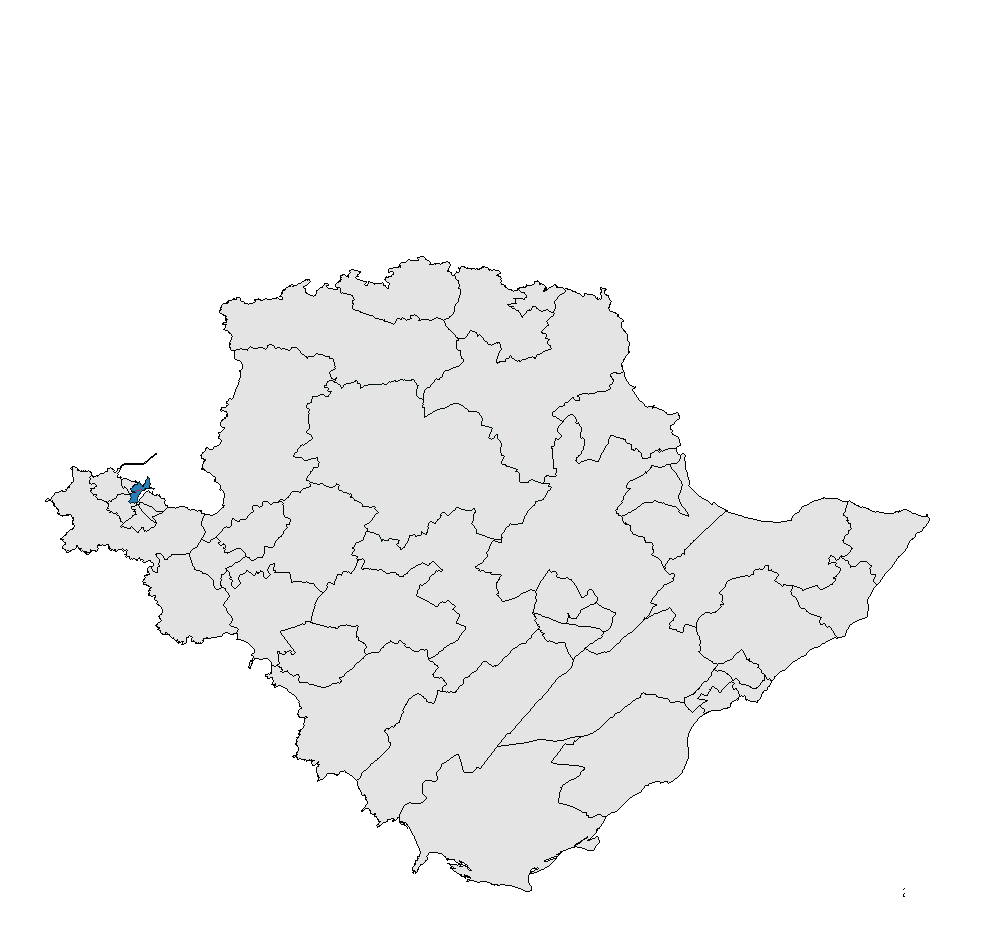
\includegraphics[width=1\linewidth]{images/ch6/mergeoverall/01}&
%\includegraphics[width=1\linewidth]{images/ch6/mergeoverall/02}&
%\includegraphics[width=1\linewidth]{images/ch6/mergeoverall/03}&
%\includegraphics[width=1\linewidth]{images/ch6/mergeoverall/04} \\
\includegraphics[width=1\linewidth]{images/ch6/mergeoverall/05}&
\includegraphics[width=1\linewidth]{images/ch6/mergeoverall/06}&
\includegraphics[width=1\linewidth]{images/ch6/mergeoverall/07}&
\includegraphics[width=1\linewidth]{images/ch6/mergeoverall/08} \\
\includegraphics[width=1\linewidth]{images/ch6/mergeoverall/09}&
\includegraphics[width=1\linewidth]{images/ch6/mergeoverall/10}&
\includegraphics[width=1\linewidth]{images/ch6/mergeoverall/11}&
\includegraphics[width=1\linewidth]{images/ch6/mergeoverall/12} \\
\includegraphics[width=1\linewidth]{images/ch6/mergeoverall/13}&
\includegraphics[width=1\linewidth]{images/ch6/mergeoverall/14}&
\includegraphics[width=1\linewidth]{images/ch6/mergeoverall/15}&
\includegraphics[width=1\linewidth]{images/ch6/mergeoverall/16} \\
\includegraphics[width=1\linewidth]{images/ch6/mergeoverall/17}&
\includegraphics[width=1\linewidth]{images/ch6/mergeoverall/18}&
\includegraphics[width=1\linewidth]{images/ch6/mergeoverall/19}&
\includegraphics[width=1\linewidth]{images/ch6/mergeoverall/20} \\
\includegraphics[width=1\linewidth]{images/ch6/mergeoverall/21}&
\includegraphics[width=1\linewidth]{images/ch6/mergeoverall/22}&
\includegraphics[width=1\linewidth]{images/ch6/mergeoverall/23}&
\includegraphics[width=1\linewidth]{images/ch6/mergeoverall/24} \\ %24
\end{tabularx}
\caption{A matrix depicting processing steps of the intermediate debug visualization for hierarchy debugging. The blue color rerpresents the most recent unified area. Grey polygons represents potential merge candidates, the red line represents the shared boundary found to unify the new area. This matrix presents the overall view of the hierarchy visualization. See Figure \ref{fig:hierarchyFocus} which shows a focus view, for clearer boundary interpretation. The file represents a test data set taken from the LSOA's of Wales, specifically the contiguous mainland of Anglesy \cite{wales}.} \label{fig:hierarchyOverall}
\end{figure}

\begin{figure}[p]
\begin{tabularx}{1\textwidth}{XXXX}
%\includegraphics[width=1\linewidth]{images/ch6/mergefocus/01}&
%\includegraphics[width=1\linewidth]{images/ch6/mergefocus/02}&
%\includegraphics[width=1\linewidth]{images/ch6/mergefocus/03}&
%\includegraphics[width=1\linewidth]{images/ch6/mergefocus/04} \\
\includegraphics[width=1\linewidth]{images/ch6/mergefocus/05}&
\includegraphics[width=1\linewidth]{images/ch6/mergefocus/06}&
\includegraphics[width=1\linewidth]{images/ch6/mergefocus/07}&
\includegraphics[width=1\linewidth]{images/ch6/mergefocus/08} \\
\includegraphics[width=1\linewidth]{images/ch6/mergefocus/09}&
\includegraphics[width=1\linewidth]{images/ch6/mergefocus/10}&
\includegraphics[width=1\linewidth]{images/ch6/mergefocus/11}&
\includegraphics[width=1\linewidth]{images/ch6/mergefocus/12} \\
\includegraphics[width=1\linewidth]{images/ch6/mergefocus/13}&
\includegraphics[width=1\linewidth]{images/ch6/mergefocus/14}&
\includegraphics[width=1\linewidth]{images/ch6/mergefocus/15}&
\includegraphics[width=1\linewidth]{images/ch6/mergefocus/16} \\
\includegraphics[width=1\linewidth]{images/ch6/mergefocus/17}&
\includegraphics[width=1\linewidth]{images/ch6/mergefocus/24}&
\includegraphics[width=1\linewidth]{images/ch6/mergefocus/18}&
\includegraphics[width=1\linewidth]{images/ch6/mergefocus/19} \\
\includegraphics[width=1\linewidth]{images/ch6/mergefocus/20}&
\includegraphics[width=1\linewidth]{images/ch6/mergefocus/21}&
\includegraphics[width=1\linewidth]{images/ch6/mergefocus/22}&
\includegraphics[width=1\linewidth]{images/ch6/mergefocus/23} \\ %24
\end{tabularx}
\caption{A matrix depicting processing steps of the debug visualization for hierarchy debugging. The blue color rerpresents the most recent unified area. Grey polygons represents potential merge candidates, the red line represents the shared boundary found to unify the new area. This matrix presents the focus view of the hierarchy visualization. Relative to Figure \ref{fig:hierarchyOverall} which depicts the same visualization using the overall focus to clearly depict progress of the process. The file represents a test data set taken from the LSOA's of Wales, specifically the contiguous mainland of Anglesy \cite{wales}.} \label{fig:hierarchyFocus}
\end{figure}

\section{Identified Errors}
Using the verification measures mentioned, we identify five majors errors that afflicted our procedure which range from user-design error to data complexities. In this Section, we present a table classifying each of these with diagrams, and discuss each one in detail with our designed solution.

\begin{table}
\footnotesize
\begin{tabularx}{\textwidth}{|m{1.5cm}|C|C|C|}
\hline
\centering Cases&Expected&Result&Modifications Made \\ \hline
\centering Non-loading polygons &  \Centerstack{\includegraphics[width=1\linewidth]{images/case-1}} Dis-joint Topology& \Centerstack{\includegraphics[width=1\linewidth]{images/case-2}} Missing Topology& Updated code to include unknown cases.\\ \hline
\centering Incorrect Contiguity & \Centerstack{\includegraphics[width=1\linewidth]{images/case-3}} Calculated Joint ~~~ Topology& \Centerstack{\includegraphics[width=1\linewidth]{images/case-4}} Calculated Dis-joint Topology& Bounding-Box Testing. \Centerstack{\includegraphics[width=0.6\linewidth]{images/ch6/AABB-AABB.png}}  ~~~ ~~~ Refer to Section \ref{sec:testing}. \\ \hline
\centering T-Junction & \Centerstack{\includegraphics[width=1\linewidth]{images/case1v3}} Joint Boundary& \Centerstack{\includegraphics[width=1\linewidth]{images/case-7}} Dis-joint interior boundary& Point-Line testing. \Centerstack{\includegraphics[width=0.8\linewidth]{images/ch6/point-line.png}} Refer to Section \ref{sec:testing}. \\ \hline
\centering Disjoint boundary edges & \Centerstack{\includegraphics[width=1\linewidth]{images/case-5}} Joint ~~~~~~~~~~~~~~~~~~~~~~~~~~ Boundary& \Centerstack{\includegraphics[width=1\linewidth]{images/case-6}} Dis-joint Exterior Boundary& Point-to-line testing, followed by edge matching via point insertion. \\ \hline
\centering  Void \& Fissures & \Centerstack{\includegraphics[width=1\linewidth]{images/case1v3.png}} Joint ~~~~~~~~~~~~~~~~~~~~~ Boundary & \Centerstack{\includegraphics[width=1\linewidth]{images/case-8.png}} Dis-joint Boundary Topology& Complete Re-design. Refer to Section \ref{sec:complex}. \\ \hline

\hline
\end{tabularx}
\caption{We present 5 error cases, comparing the expected result to the error that we produced using simple diagrams.}
\end{table}


\subsection{Non-Loading Polygons}
Adding visualization techniques to this step was more important than is first apparent. We used open source library Geospatial Data Abstraction Library (GDAL) \cite{GDAL} to load shapefiles. However, we noticed that during the representation of geospatial data, some areas would not load, which we learned using comparative software, QGIS. It was clear the general shape of maps differed between our software and our comparitive software. Using loading verification, we found data was not being loaded from the file, rather than it being lost or corrupted in some processing steps. This was due to the mishandling of polygon types due to the way GDAL handles ``polygons'' and ``multi-polygons'' seperately. ``Inner'' rings, as labeled by GDAL, caused a second challenge that we ran into. They are used to separate internal area's vertex lists from those of the primary outer boundary. Although the problem was identified later using visualization concepts, we noticed that inner rings were not represented in the loading visualization step. After further research, we found the additional vertex lists. Refer to Figure \ref{fig:rings} for an example.


These mistakes may have been avoided by a more experienced user of the library, but geospatial debug visualization proved an essential tool for new users.

\begin{figure}[t]
\includegraphics[width=0.4\linewidth]{images/ch6/innerRings}
\caption{Two examples of inner rings, highlighted in yellow. These can be found in the Lower Super Output Areas (LSOAs) of Wales in ``Carmarthenshire'' \cite{wales}.} \label{fig:rings}
\end{figure}

\subsection{Incorrect Contiguities} \label{sec:contigVis}
Contiguity became an important step in our understanding of contiguous regions. As it presents the first complexities associated with working on real-world ShapeFiles. The debug process first diagnosed a flaw in our boundary box testing with margin of error. When initially creating our checked, it seemed like a smart idea to set up margins of error to allow when identifying potential neighbours. The scale of Shape Files can vary wildly, moving from a scale of 200, to scale of 200,000, and not limiting itself positive coordinate spaces. Because of this, there were a lot of complications with with defining a global margin of error. In the end, we reduce completexity to encourage rigid testing. Our bounding box tests are discussed in Section \ref{sec:testing}.

\subsection{T-Junctions}
The T-Junction error occurs within a pre-existing merged area. This is caused when a shared boundary's vertices do not line up with a point that may be used on a later shared boundary.
Figure \ref{fig:t-junction} (on Page \pageref{fig:t-junction}) is an example of such an occurence. Since the T-junction point is considered a non-shared boundary point, the boundary ends, and since the next boundary is a part of the shared boundary, the algorithm would mistake most of the vertices as the shared boundary. Once identified, we added the option to include point-to-line tests within a shared boundary. Although this would reduce performance time, we rectify this with the ability to save and load build instructions which speed up performance during a later run of a shape file. We discuss of point-to-line testing in Section \ref{sec:testing}.

\begin{figure}[b]
\includegraphics[width=0.5\textwidth]{images/ch6/t-junctoZoom2}
\caption{A depiction of disjoint edges. Green dotted lines signify standard boundary matching.  Red boundary refers to disjoint edges matched due to the point-to-line tests. Polygons seperated for clarity. }\label{fig:t-junction}
\end{figure} 

\subsection{Disjoint Boundary Edges}
Related to our first issue, the dis-joint boundary edges begun to become visible when the point-to-line tests were intergrated into boundary testing. An example can be foubd in Figure \ref{fig:weirdBoundary} (on Page \pageref{fig:weirdBoundary}). The cause of the error refers to sections where the end of a boundary occur on different sections, where a t-junction occurs at the edge of a boundary. Now that point-to-line tests were used, the boundary tests would move a step further than usual, causing the area with no points to remove an unrelated point. In order to fix this, our point-to line test was followed by a section to import our vertex into it's neighbour as the new final vertex. The error was identified using our focus processing step, which enables the user to see minor errors in boundary design.

\begin{figure}
\includegraphics[width=1\textwidth]{images/ch6/currentProblem}
\caption{The red color represents the assumed shared boundary. The first instance of the T-junction challenge discussed in more detail in Chapter \ref{chap:dcm}.  Using the debug visualization for hierarchy building, along with comparative software tools, we were able to identify the exact vertex point (circled green) that caused the problem. This Lead us to re-evaluate the handling of T-junctions. We identify the boundary as the introduction between the following areas within a LSOA of Wales test data set in the ``Isle of Anglesey'' \cite{wales}. }\label{fig:t-junction}
\end{figure} 
\begin{figure}
\includegraphics[width=1\textwidth]{images/ch6/WeirdBoundary3}
\caption{ The first instance of shared boundary matching. The red shared boundary refers to the assumed shared boundary. the blue color refers to the focus area, the background color is represented by the dark grey. The red boundary seems to stop just short of the shared boundary, however there are no vertex points to join at the end causing an error. After dscovering this, the algorithm was upgraded to check both sides of a shared boundary and match them using a point-to-line intersection. We highlight the problem with a green circle. }\label{fig:weirdBoundary}
\end{figure} 

\subsection{Voids and Fissures} \label{sec:complex}
The next case  we look at is caused by what we call a fissure, which refers to space between boundary vertices. Although we considered voids as single anomalies along a shared boundary, learning that it was common to have a set of continuous voids (caused by rivers or mountains) made it impossible to ignore these anomalies. This lead us to an extensive re-factoring of the algorithm, that was used to diagnose the difference between these voids, and a non-shared boundary. Figures \ref{fig:errorVoids} \& \ref{fig:splitBoundary} on Pages \pageref{fig:errorVoids} \& \pageref{fig:splitBoundary} Present in-situ examples found using our debug visualization.

Correctly identifying boundaries was one of the biggest challenges througout the course of the PhD. There are many considerations that are necessary to create a robust procedure which can be used. In order to explain some of these challenges, this section covers some of our previous attempts and the road blocks that we encountered. For our first attempt, we implemented a simple vertex matching algorithm. For a merge pair, we test each vertex against every other vertex for overlap. Common vertices would be saved to a seperate vertex list and this was used to remove those vertices from both areas to identify a shared boundary. There were two shortcomings with this approach.


\subsubsection{Unification of Area Pair}
The first challenge is identification of a boundary seemed simple, but unifying the two areas along this boundary is more difficult. In order to unify the merge pair along with their non-shared boundary, it is necessary to identify where in the vertex list the boundaries originates. In order to reconcile this, we made some changes to the original implementation. First, we saved the identity of the beginning and ending points of a shared boundary. This enables us to recognize where and when we need to unify the two areas. The second change we make is to control vertex direction. This enables us to increase identification of unification order as follows: $P_aOrigin->P_aStart->P_bEnd->P_bStart->P_aEnd->P_aOrigin$. Refer to Figure \ref{fig:attempt1}.

The challenge with this assumption is with the origin. At this point, we assume that the origin is not already on the shared boundary. This is not always the case. A shared boundary can span an arbitrary number of vertices, and can also be positioned at any point within the vertex list. This means that a start vertex can reside within the shared boundary. In order to rectify this situation, we order the vertex list of the merge pair in order to pre-emptively sort the vertex list. When we diagnose the end of a shared boundary, we make this the beginning of the non-shared boundary. Refer to Figure \ref{fig:attempt2}.

\begin{figure}[t]
\subfloat{\includegraphics[width=0.4\linewidth]{images/ch6/attemptA}\label{fig:attempt1}}~~ 
\subfloat{\includegraphics[width=0.4\linewidth]{images/ch6/attemptB}\label{fig:attempt2}}
\caption{(left) Our first attempt to unify areas. (right) The improved process to unify areas. We re-order the vertex list to start at the end of a shared boundary.} 
\end{figure}


\subsubsection{Identifying the Start and End of a Shared Boundary}
Now that we understand why finding the start and end of a shared boundary is critical, we discuss the challenges for finding these start and end points. Attempting to use our previous procedure to identify common vertices is not appropriate, although we did not fully understand why up to this point. This was due to voids and fissures in the non-shared boundary. Because of the frequency of these configurations, they gained an accumulative effect on further identification processes which caused the early versions of the algorithm to crash. At this point, we had not implemented debug visualization to inform the cause of the errors. However, we did identify what we considered as rendering errors, points along the shared boundary that were still rendered (which were later identified as voids and fissures, causing error at later cycles).

\begin{figure}[t]
%\includegraphics[width=1\textwidth]{images/ch6/attempt1p2}
\includegraphics[width=1\textwidth]{images/ch6/caseA}
\caption{The second version of our boundary identifier using a bi-directional search. We identify two cases, Case A refers to the origin ($V_0$) residing on a non-shared boundary whilst Case B refers to the origin ($V_0$) residing on a shared boundary. The arrows refer to the direction tested and length of the clockwise or anti-clockwise search.} \label{fig:searchA}
\end{figure}

In order to rectify these errors, we modified our extraction algorithm to include a bi-directional search. From the origin, we search both clockwise and anti-clockwise. In this case, we can assume that the route can fall into two cases. First the origin resides on a non-shared boundary. If this is the case (Case A, Figure \ref{fig:searchA}), we search bi-directionally if the clockwise search encounters a common vertex, we can use that as the start of the shared boundary whilst the first common vertex in the anticlockwise search will be considered the end of the shared boundary. The second case (Case B, Figure \ref{fig:searchA}) is if we start on a shared boundary. In this case, our configuration can be flipped, where the last common vertex before a non-common vertex in the anti-clockwise direction is the start of the shared boundary, and the last common vertex before a non-common vertex in the clockwise position is the end of the shared boundary. However, this approach also falls apart when we add new exceptions. Refer to Figure \ref{fig:searchA} for a visual representation.


The first condition we found was a T-junction. In order to verify a non-common vertex is not part of a shared boundary, we now have to test if this point falls on a line segment. This increases the complexity of common vertex testing, but the algorithm handles this exception well. The second exception is more of a challenge. We now detect voids which we describe as an extra point on a shared boundary that does not lie on shared boundary line. This complicates Case B, as now we cannot consider the first non-common vertex to accurately depict the start or end of a boundary. For this, we added void tests, to see if the shared boundary contiuned. The other challenge with a void is that it now has potential to falsely identify the Case B as case A. If the start vertex falls on a void, the algorithm would assume that we now sit within Case A (Case A of figure \ref{fig:searchB}) which presents a false postive boundary selection.

 This becomes more complex when you consider fissures which feature an arbitrary number of linked voids, allowing for more oppurtunities for this exception to present itself, and nullifies any void testing which could be used to depict it. Finally we also find examples of voids and fissures with multiple instances within one shared boundary to complicate this. Refer to Figure \ref{fig:searchB} for a visual representation.
 
 \begin{figure}[t]
%\includegraphics[width=1\textwidth]{images/ch6/attempt2p2}
\includegraphics[width=1\textwidth]{images/ch6/caseB}
\caption{Errors that occur when voids are considered. We run the same cases (A and B) from Figure \ref{fig:searchA} and implement voids which causes two distinct errors. As voids can be replaced with fissures, and can be found multiple times. This represents only the simplest cases for error. Case A begins on a void, while Case B holds a void on the shared boundary.} \label{fig:searchB}
\end{figure}

In Chapter \ref{chap:dcm}, we discuss the fact that over 50\% of one of our test cases contain voids, T-junctions, or fissures, when identifying a shared boundary. This causes a major concern when identifying shared boundaries. We could have cleaned the shapefiles of voids and fissures, however the shape files we work with are considered industry standard. It would be disingenuous to believe that our algorithm is useful when we hold the only shapefiles that the algorithm worked with.



In order to rectify this problem, we added two hueristics, and develop a more advanced method.
First, we assumed that boundaries between two areas are not split, and are one contiguous boundary. Split shared boundaries between areas are already rare, however, we made this assumption due to our focus on scale. Our algorithm's distance metric is biased towards merging the smallest area with it's smallest neighbour. Even amongst cases where a split boundary could occur, it would be highly irregular for a boundary that caused a split boundary to not be considered the first area to be merged. 
Our second assumption is that a shared boundary has a shorter length than a non-shared boundary. It is more likely for this to occur, however just like with our first assumption, we mitigate the chances of our assumption being false by considering the smallest neighbour above others. See Figure \ref{fig:length}.

\begin{figure}[hb]
%\includegraphics[width=1\textwidth]{images/ch6/attempt2p2}
\includegraphics[width=1\textwidth]{images/ch6/length}
\caption{Depiction of topological distance test of non-shared boundaries for a non-void vertex list. We search the list as loops until all vertexes have been tested.} \label{fig:length}
\end{figure}

\begin{figure}
\includegraphics[width=1\textwidth]{images/ch6/multipleVoids3}
\caption{This presents a focused step presenting an error that occurred in the processing of the geospatial data. The red line presents the assumed shared boundary, the white presents a context polygon, the grey represents the default background, and the blue signifies the unified polygon. This error was caused by a fissure along the shared boundary which result in a unification error. This is because an early version of our algorithm assumed that voids would only occur in singular instances. The fissure made the logic believe we rejoined a shared boundary shape, causing most of the boundary to be lost in the unification process, depicted by the straight red line moving off the right size of the canvas which then meets up to complete a loop (see Figure \ref{fig:t-junction} to see an example of how the boundary loops). Refer to Figure \ref{fig:splitBoundary} for the location and cause, where we match the areas using a green circles.} \label{fig:errorVoids}
\end{figure}

\begin{figure}
\includegraphics[width=1\textwidth]{images/ch6/BoundarySplit2}
\caption{This is a screenshot taken from QGIS to verify an error found in Figure \ref{fig:errorVoids} The polygons contain a strange break in between them which was only visible at a 1:14 scale of the original data set. Something that would be impossible to identify if reviewing the data as an overview image. The white is the background of the software, signifying a lack of any polygonal data. The green circle relates to a point relative to the green circle in Figure \ref{fig:errorVoids}. The void is so thin that we can not clearly identify the all the voids in one image. 
This error occured between the community wards of "Cynghordy" and "Rhandirmwyn" \cite{ONS}.
 } \label{fig:splitBoundary}
\end{figure}

\section{Intersection Testing for Primitives} \label{sec:testing}
Intersection testing is one of the key areas that we examine when reviewing performance. Two tests, in particular, result in a high frequency of calls: the point-to-line and bounding box intersection test. The first is used as a deep search into accurate boundary representation, while the second is a filter for disjoint, non-intersecting polygons. Although there are many methods online to help manage these tests, we did not find a developer-friendly library that managed to guide us with primitive testing. Therefore, we created a small open-source library to test the intersection between five different primitives. The primitives we test are:
\begin{itemize}
\item Point - Defined as an (x, y) coordinate, $p(x,y)$
\item Line Segment - Defined as two points (assumed to be connected), ($p_1,p_2)$)
\item Circle -  Defined by a center point, and a radius, ($p_c,r)$)
\item Triangle - Defined by three points ($p_1,p_2,p_3$)
\item Axis-Aligned Bounding Box (AABB) - Defined by four points, assumed to be aligned.
\end{itemize}

Other than the triangle, which is added for completeness, all of these tests are necessary for the software project. Points are used to present vertices, as well as the mouse pointer, Line Segments are used to test precise boundaries for shared boundary testing, circles are used to test likely collision with glyphs, and axis-aligned bounding boxes are used to test possible collisions with boxes. We present this as an open source project (Section \ref{sec:open}).

\subsection{Motivation}
Generic shape intersection testing is a major component within the algorithm presented in this thesis. We present a table depicting meta data for different tested shape files, and the number of intersection tests we gathered for some of our tests. See Table \ref{tbl:tests}. For this table, we present a number of examples that are used in Chapters \ref{chap:dcm}, \ref{chap:userStudy} \& \ref{chap:MultivariateMaps}. Polygon Count records the AABB-to-AABB tests, whilst the vertex count records the Point-to-Line tests.

\begin{table}[b]
\footnotesize
\ra{0.95}
\rowcolors{1}{black!10}{white}
\begin{tabularx}{1\linewidth}{|CCC|CCC|}
\hline
\multicolumn{3}{|c|}{\textbf{Meta Data}} & \multicolumn{3}{c|}{\textbf{Intersection Tests}}\\ \hline
ShapeFile Name&Polygon Count&Vertex Count& Point-to-Line (\% of tests) & ABBB-to-AABB (\% of tests)&Total Tests\\ \hline \footnotesize
CCGs& 541	&2,890,934	&5,208,849 (99\%)		&52,284 \newline (1\%)		&5,261,133 \\ 
Ahupuaa Boundaries of Hawaii & 725 & 284,252 & 547,303 (70\%) & 239,024 (30\%) & 786,327 \\
LSOA of Wales & 1,949 &2,417,391 & 4,648,604 (80\%) & 1,175,523 (20\%) & 5,824,127 \\ 
US Counties& 3,134&51,976	&126,841 \newline (6\%)	&2,007,756 (94\%)	&2,134,597 \\ 
Republic of Ireland Electoral Divisions& 4,407		&419,368	&935,468 (16\%)	&4,742,824 (84\%)	&5,678,292\\ 
Germany & 5,385 & 1,456,469 & 6,287,363 (38\%)& 10,093,710 (62\%) & 16,381,073\\
Italy & 8,946 & 966,206 &1,463,588 (4\%) &31,817,661 (96\%)&33,281,249 \\ 
Brazil & 11,181 & 1,288,007 & 6,124,539 (11\%)& 47,995,943 (89\%) & 54,120,482\\ 

\hline
\end{tabularx}
\caption{A table recording some results for intersecting testing. We record the two major tests from the examples in Chapter \ref{chap:MultivariateMaps} as well as a few more represented in Chapters \ref{chap:dcm} and \ref{chap:userStudy}.} \label{tbl:tests}
\end{table}

\subsection{Graphical User Interface}
In order to present our library header, the files includes a graphical user interface for testing purposes using Qt \cite{Qt}. The user can select any of the primitives to move using their mouse with a dropdown box and create a static primitive to test against using a second  dropdown box. See Figure \ref{fig:inter}.
\begin{figure}[t]
\subfloat[No Intersection]{
\includegraphics[width=0.48\linewidth]{images/ch6/noInter}}
\subfloat[Intersection]{
\includegraphics[width=0.48\linewidth]{images/ch6/inter}}
\caption{Sample image representing the intersection tester GUI. (a) refers to an example of no intersection, while (b) presents an example of an intersection. When an intersection occurs, the primitives change to green.} \label{fig:inter}
\end{figure}

\subsection{Using Primitives}
The library provides classes for each primitive with basic functionality. The idea behind this library is that testing for intersections is simple. Objects are created or cast into our own primitive objects, and the function \emph{isIntersecting(Object a, Object b)}, returns a boolean value. Although this library is used within our project, we also provide a graphical user interface using Qt to test the library. This enables us to test each primitive against any other primitive conveniently.
\newpage
\lstinputlisting[language=c++]{src/simpleTest.cpp}

We also give the user access to more information for their own testing. For example, we use a method to test the closest point on a line, to a second point. Rather this allows the user to find that point and make other tests. For example, in our Graphical User Interface, we depict the closestPoint while testing some primitives.
\lstinputlisting[language=c++]{src/closestPoint.cpp}

\subsection{Open Source} \label{sec:open}
In order to maximize the potential of this library, we upload a public copy to GitHub. The library can be found with the two main headers, the GUI testing project, test cases and full Doxygen documentation \cite{van2008doxygen}. We plan to update this in the future with any performance optimzations, and additional shapes that may be necessary. We also hope to include 3D functionality in the future as well as other shapes. As well as some extra return procedures for the point(s) of intersection, or points clamped outside of the primitives. This can be found at \url{https://github.com/liammcnabb/IntersectionTester}.

\section{Conclusion}
In this Chapter, we discuss many of the aspects related to debugging our geospatial visualization effectively. We first present debug visualization concepts, and our own personalized debug visualizations, we classify the major errors that were encountered with in-system identification, and discuss how we rectified these issues. Finally, we discuss our primative testing library, and where it can be found.

